\documentclass[11pt]{beamer}
\usepackage{graphicx}
\usepackage[export]{adjustbox}  % max width/height in includegraphics
\usepackage[framemethod=TikZ]{mdframed}
\usepackage[document]{ragged2e}

%\usepackage{soul}
\usepackage{xcolor}
\usepackage{ifthen}
\usepackage{fontspec}
%\usepackage{textcomp}
%\usepackage[T5,T1]{fontenc}
\usepackage{caption}


\usetheme[hideothersubsections]{Goettingen}
\usecolortheme{seahorse}
%%% \usetheme{Montpellier}
%%% \usecolortheme{dolphin}
\setbeamercovered{invisible}
\setbeamertemplate{navigation symbols}{\insertslidenavigationsymbol}
\setbeamertemplate{page number in head/foot}{}
\setbeamertemplate{blocks}[rounded][shadow=false]
% \setbeamerfont{section in sidebar}{size=\fontsize{4}{3}\selectfont}
% \setbeamerfont{subsection in sidebar}{size=\fontsize{4}{3}\selectfont}
% \setbeamerfont{subsubsection in sidebar}{size=\fontsize{4}{2}\selectfont}


% workaround for problem that causes shadows on rounded corners to not look right
\makeatletter
\def\pgfutil@insertatbegincurrentpagefrombox#1{%
  \edef\pgf@temp{\the\wd\pgfutil@abb}%
  \global\setbox\pgfutil@abb\hbox{%
    \unhbox\pgfutil@abb%
    \hskip\dimexpr2in-2\hoffset-\pgf@temp\relax% changed
    #1%
    \hskip\dimexpr-2in-2\hoffset\relax% new
  }%
}
\makeatother


\usepackage{microtype}
% \DisableLigatures[f]{encoding = *, family = *}

%% languages and fonts
% \usefonttheme{professionalfonts} % using non standard fonts for beamer
\usepackage{tgheros}
\usefonttheme{serif}
\usepackage{XCharter}

%\usepackage{xeCJK}
%\usepackage{textgreek}
% \usepackage{polyglossia}
% \setdefaultlanguage{english}
% \setotherlanguage{russian}
% \newfontfamily\russianfont{/System/Library/Fonts/Times.ttc}
% \let\russianfonttt\ttfamily

% \setCJKmainfont{/System/Library/Fonts/STHeiti Light.ttc}
% \setCJKmonofont{/System/Library/Fonts/PingFang.ttc}
% \setCJKsansfont{/System/Library/Fonts/PingFang.ttc}


\AtBeginSection[]{
  \begin{frame}
    \vfill
    \centering
    \begin{beamercolorbox}[sep=8pt,center,shadow=true,rounded=true]{title}
    \usebeamerfont{title}\insertsectionhead\par%
    \ifthenelse{\equal{\thisSectionName}{Bonus}}{}{
        \usebeamerfont{subtitle}\thisSectionName\par%
    }
    \end{beamercolorbox}
    \ifthenelse{\equal{\thisSectionName}{Bonus}}
    {
        \vspace*{.5em}
        Get ready for some \emph{devilishly} hard questions!
        \vspace*{.5em}
    }{}
    \begin{center}
    \ifthenelse{\equal{\thisSectionName}{Bonus}}{
        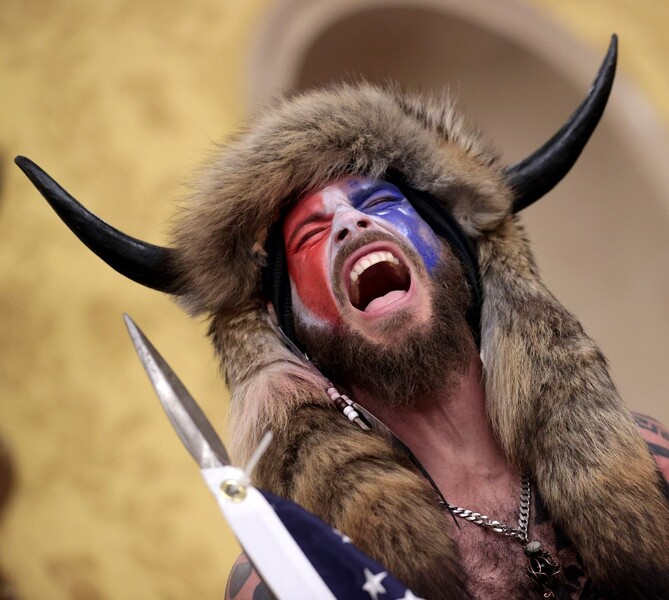
\includegraphics[max height = 0.3\textheight]{Images/qshaman.jpeg}

        \vspace*{.5em}

        (Here's some trivia: This particular devil actually lives with his mother.)
    }{}

    \vspace*{.9em}
    Please mute yourselves!
    \end{center}


    \vfill
  \end{frame}
}

\AtBeginSubsection[]{
  \begin{frame}
    \vfill
    \centering
    \begin{beamercolorbox}[sep=8pt,center,shadow=true,rounded=true]{title}
    \usebeamerfont{title}\insertsectionhead\par%
    \usebeamerfont{subtitle}\insertsubsectionhead\par%
    \end{beamercolorbox}
    \ifthenelse{\equal{\subsecname}{Answers}} {
        \begin{center}
        Unmute yourselves!
        \end{center}
    }
    \vfill
  \end{frame}
}
\begin{document}

\title{Welcome to Quarantine Trivia XIV!}
\date{}

\begin{frame}
\titlepage{}
\begin{center}

\includegraphics[max width=0.9\textwidth,
    max height=0.4\textheight]{Images/triviatitleframelogo.png}
\end{center}
\end{frame}

\begin{frame}[t]{Question 1}
\vspace{-0.5em}
\begin{block}{Question}
Which player's birthday is today?
\end{block}

\visible<2->{
    \begin{block}{Answer}
    Kathleen O'Keefe. Happy birthday, Kathleen!
    \end{block}
}
\end{frame}

\begin{frame}
This week, we couldn't resist putting a trivia spin on the prevailing meme.
\pause
\begin{center}
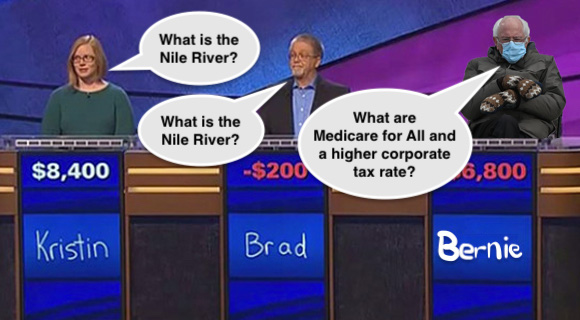
\includegraphics[max width=.95\textwidth,
max height=0.55\textheight]{Images/bernie.jpg}
\end{center}
\end{frame}

\begin{frame}
And one last thing before we begin: By the end of this game, you will have answered
over 1,500 trivia questions.
\pause
\\
\bigskip
(And by our estimation, almost 100 of them were not \mbox{challenged}.)
\end{frame}

\begingroup{}
\begingroup{}
\begin{frame}[t]{Categories}
This week, you'll be answering questions in the following categories:
\begin{enumerate}
\item .org
\item Answer Like It's 1999
\item Count On It
\item Ham's Solo
\item Philosophy and Philosophers
\item Planet Earth
\item Scandalous Literature
\item The ``Mother of Presidents''
\item Who Directed It?
\item ``Royals''
\item Bonus Round
\end{enumerate}
\end{frame}
\endgroup{}

\begingroup{}
\begin{frame}
\vfill{}
\begin{beamercolorbox}[sep=8pt,center,shadow=true,rounded=true]{title}
\usebeamerfont{title}Good luck everyone! And have fun!
\end{beamercolorbox}
\vfill{}
\end{frame}
\endgroup{}
\def\thisSectionName{.org}
\section{Round 1}
\subsection*{Q1}
\begin{frame}[t]{Round 1 --- .org --- \mbox{Question 1}}
\vspace{-0.5em}
\begin{block}{Question}
What is the name of the organization dedicated to  the protection of marine life, one of whose ships was named the Rainbow Warrior?
\end{block}
\end{frame}
\subsection*{Q2}
\begin{frame}[t]{Round 1 --- .org --- \mbox{Question 2}}
\vspace{-0.5em}
\begin{block}{Question}
What is the name of the organization with which Jimmy Carter has long been associated that helps provide people with affordable housing by building and repairing homes?
\end{block}
\end{frame}
\subsection*{Q3}
\begin{frame}[t]{Round 1 --- .org --- \mbox{Question 3}}
\vspace{-0.5em}
\begin{block}{Question}
What is the full name of the organization known as UNICEF\@?
\end{block}
\end{frame}
\subsection*{Q4}
\begin{frame}[t]{Round 1 --- .org --- \mbox{Question 4}}
\vspace{-0.5em}
\begin{block}{Question}
Which charitable organization is actually a religion whose adherents have military titles?
\end{block}
\end{frame}
\subsection*{Q5}
\begin{frame}[t]{Round 1 --- .org --- \mbox{Question 5}}
\vspace{-0.5em}
\begin{block}{Question}
wish.com is an online e-commerce site. Which organization's site is wish.org?
\end{block}
\end{frame}
\subsection*{Q6}
\begin{frame}[t]{Round 1 --- .org --- \mbox{Question 6}}
\vspace{-0.5em}
\begin{block}{Question}
What organization that is headquartered at New York City's Bronx Zoo works to protect the world's wild places?
\end{block}
\end{frame}
\subsection*{Q7}
\begin{frame}[t]{Round 1 --- .org --- \mbox{Question 7}}
\vspace{-0.5em}
\begin{block}{Question}
Which foundation founded in 1997 has its offices in New York City and Little Rock, Arkansas?
\end{block}
\end{frame}
\subsection*{Q8}
\begin{frame}[t]{Round 1 --- .org --- \mbox{Question 8}}
\vspace{-0.5em}
\begin{block}{Question}
What famous U.S. organization is dedicated to keeping your vena cavas and ventricles working properly?
\end{block}
\end{frame}
\subsection*{Q9}
\begin{frame}[t]{Round 1 --- .org --- \mbox{Question 9}}
\vspace{-0.5em}
\begin{block}{Question}
Which .org helps you evaluate charities (it might be said to help you chart your course through them)?
\end{block}
\end{frame}
\subsection*{Q10}
\begin{frame}[t]{Round 1 --- .org --- \mbox{Question 10}}
\vspace{-0.5em}
\begin{block}{Question}
What organization that was founded in the UK in 1919 is dedicated to improving the lives of children?
\end{block}
\end{frame}
\subsection{Answers}
\begin{frame}[t]{Round 1 --- .org --- \mbox{Answer 1}}
\vspace{-0.5em}
\begin{block}{Question}
What is the name of the organization dedicated to  the protection of marine life, one of whose ships was named the Rainbow Warrior?
\end{block}

\visible<2->{
    \begin{columns}[T,totalwidth=\linewidth]
    \begin{column}{0.32\linewidth}
    \begin{block}{Answer}
    Greenpeace
    \end{block}
    \end{column}
    \begin{column}{0.65\linewidth}
    \begin{center}
    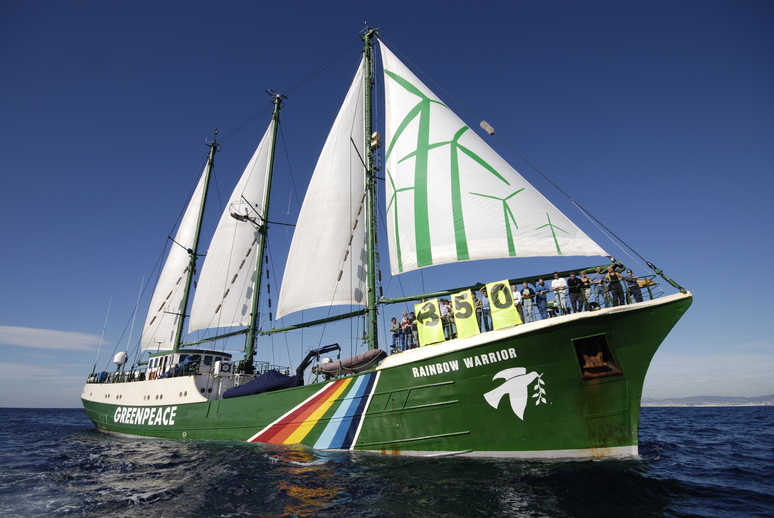
\includegraphics[max width=0.95\textwidth,
        max height=0.48000\textheight]{{Images/greenpeace}.jpg}
    \end{center}
    \end{column}
    \end{columns}
}
\end{frame}
\begin{frame}[t]{Round 1 --- .org --- \mbox{Answer 2}}
\vspace{-0.5em}
\begin{block}{Question}
What is the name of the organization with which Jimmy Carter has long been associated that helps provide people with affordable housing by building and repairing homes?
\end{block}

\visible<2->{
    \begin{columns}[T,totalwidth=\linewidth]
    \begin{column}{0.32\linewidth}
    \begin{block}{Answer}
    Habitat for Humanity
    \end{block}
    \end{column}
    \begin{column}{0.65\linewidth}
    \begin{center}
    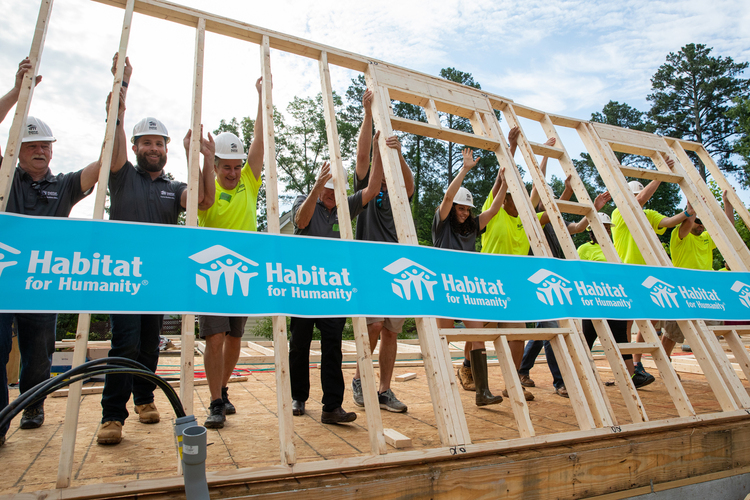
\includegraphics[max width=0.95\textwidth,
        max height=0.43000\textheight]{{Images/habitat}.jpg}
    \end{center}
    \end{column}
    \end{columns}
}
\end{frame}
\begin{frame}[t]{Round 1 --- .org --- \mbox{Answer 3}}
\vspace{-0.5em}
\begin{block}{Question}
What is the full name of the organization known as UNICEF\@?
\end{block}

\visible<2->{
    \begin{columns}[T,totalwidth=\linewidth]
    \begin{column}{0.65\linewidth}
    \begin{block}{Answer}
    United Nations Children's Fund / United Nations International Children's Emergency Fund (``International'' and ``Emergency'' were part of the original name, but have since been dropped)
    \end{block}
    \end{column}
    \begin{column}{0.3\linewidth}
    \begin{center}
    
\includegraphics[max width=0.95\textwidth,
        max height=0.53000\textheight]{{Images/unicef}.jpg}
    \end{center}
    \end{column}
    \end{columns}
}
\end{frame}
\begin{frame}[t]{Round 1 --- .org --- \mbox{Answer 4}}
\vspace{-0.5em}
\begin{block}{Question}
Which charitable organization is actually a religion whose adherents have military titles?
\end{block}

\visible<2->{
    \begin{columns}[T,totalwidth=\linewidth]
    \begin{column}{0.32\linewidth}
    \begin{block}{Answer}
    The Salvation Army (the religion is the Salvationist religion)
    \end{block}
    \end{column}
    \begin{column}{0.65\linewidth}
    \begin{center}
    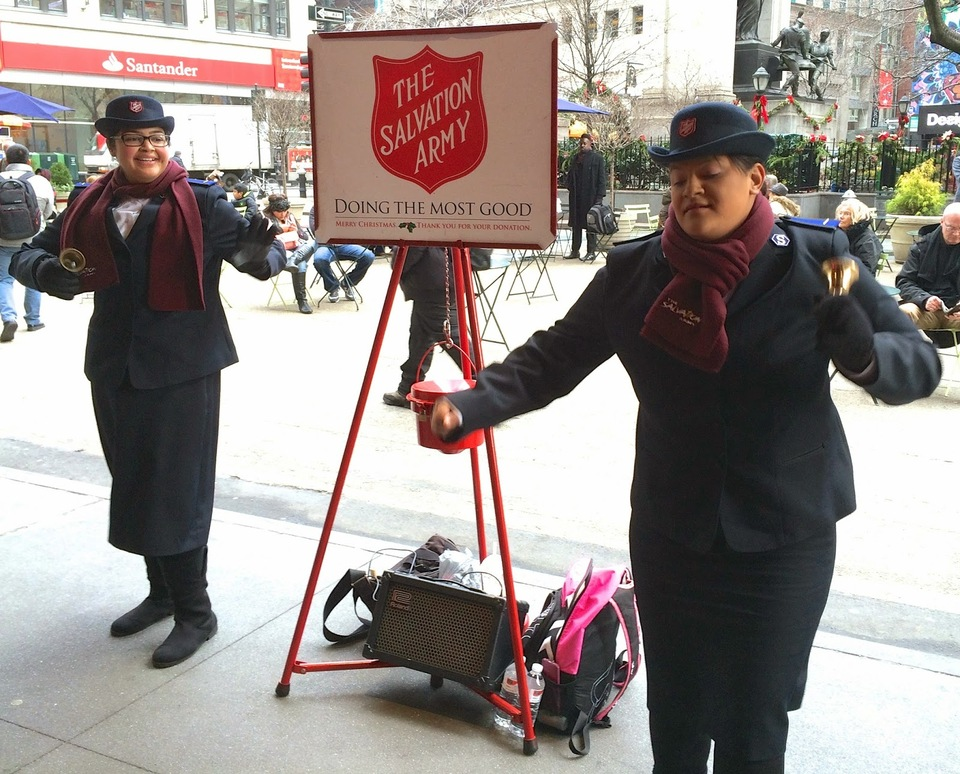
\includegraphics[max width=0.95\textwidth,
        max height=0.53000\textheight]{{Images/salvation}.jpg}
    \end{center}
    \end{column}
    \end{columns}
}
\end{frame}
\begin{frame}[t]{Round 1 --- .org --- \mbox{Answer 5}}
\vspace{-0.5em}
\begin{block}{Question}
wish.com is an online e-commerce site. Which organization's site is wish.org?
\end{block}

\visible<2->{
    \begin{columns}[T,totalwidth=\linewidth]
    \begin{column}{0.32\linewidth}
    \begin{block}{Answer}
    Make-a-Wish / The Make-a-Wish Foundation
    \end{block}
    \end{column}
    \begin{column}{0.65\linewidth}
    \begin{center}
    
\includegraphics[max width=0.95\textwidth,
        max height=0.53000\textheight]{{Images/makeawish}.jpg}
    \end{center}
    \end{column}
    \end{columns}
}
\end{frame}
\begin{frame}[t]{Round 1 --- .org --- \mbox{Answer 6}}
\vspace{-0.5em}
\begin{block}{Question}
What organization that is headquartered at New York City's Bronx Zoo works to protect the world's wild places?
\end{block}

\visible<2->{
    \begin{columns}[T,totalwidth=\linewidth]
    \begin{column}{0.32\linewidth}
    \begin{block}{Answer}
    The Wildlife Conservation Society
    \end{block}
    \end{column}
    \begin{column}{0.65\linewidth}
    \begin{center}
    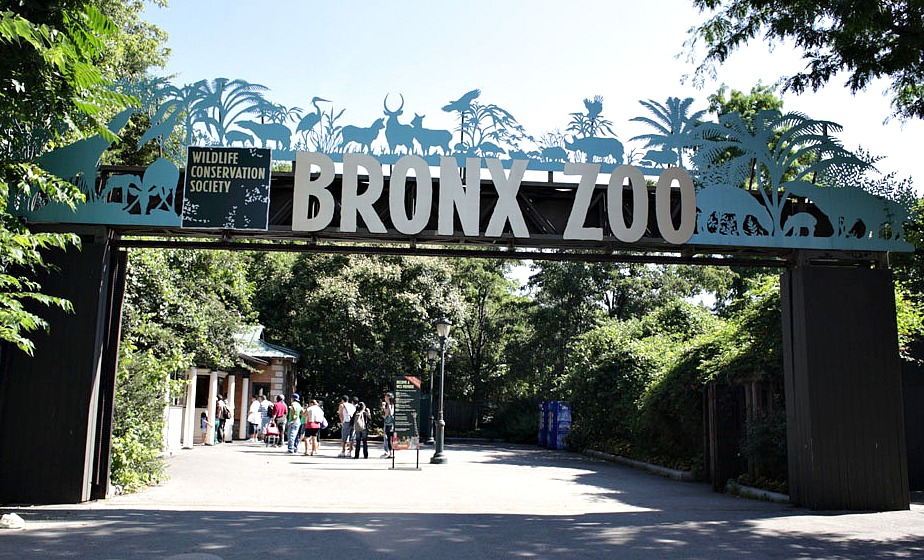
\includegraphics[max width=0.95\textwidth,
        max height=0.48000\textheight]{{Images/wcs}.jpg}
    \end{center}
    \end{column}
    \end{columns}
}
\end{frame}
\begin{frame}[t]{Round 1 --- .org --- \mbox{Answer 7}}
\vspace{-0.5em}
\begin{block}{Question}
Which foundation founded in 1997 has its offices in New York City and Little Rock, Arkansas?
\end{block}

\visible<2->{
    \begin{columns}[T,totalwidth=\linewidth]
    \begin{column}{0.32\linewidth}
    \begin{block}{Answer}
    The Clinton Foundation
    \end{block}
    \end{column}
    \begin{column}{0.65\linewidth}
    \begin{center}
    
\includegraphics[max width=0.95\textwidth,
        max height=0.53000\textheight]{{Images/clinton}.png}
    \end{center}
    \end{column}
    \end{columns}
}
\end{frame}
\begin{frame}[t]{Round 1 --- .org --- \mbox{Answer 8}}
\vspace{-0.5em}
\begin{block}{Question}
What famous U.S. organization is dedicated to keeping your vena cavas and ventricles working properly?
\end{block}

\visible<2->{
    \begin{columns}[T,totalwidth=\linewidth]
    \begin{column}{0.32\linewidth}
    \begin{block}{Answer}
    American Heart Association
    \end{block}
    \end{column}
    \begin{column}{0.65\linewidth}
    \begin{center}
    
\includegraphics[max width=0.95\textwidth,
        max height=0.48000\textheight]{{Images/americanheart}.png}
    \end{center}
    \end{column}
    \end{columns}
}
\end{frame}
\begin{frame}[t]{Round 1 --- .org --- \mbox{Answer 9}}
\vspace{-0.5em}
\begin{block}{Question}
Which .org helps you evaluate charities (it might be said to help you chart your course through them)?
\end{block}

\visible<2->{
    \begin{columns}[T,totalwidth=\linewidth]
    \begin{column}{0.32\linewidth}
    \begin{block}{Answer}
    Charity Navigator
    \end{block}
    \end{column}
    \begin{column}{0.65\linewidth}
    \begin{center}
    
\includegraphics[max width=0.95\textwidth,
        max height=0.48000\textheight]{{Images/navigator}.jpg}
    \end{center}
    \end{column}
    \end{columns}
}
\end{frame}
\begin{frame}[t]{Round 1 --- .org --- \mbox{Answer 10}}
\vspace{-0.5em}
\begin{block}{Question}
What organization that was founded in the UK in 1919 is dedicated to improving the lives of children?
\end{block}

\visible<2->{
    \begin{columns}[T,totalwidth=\linewidth]
    \begin{column}{0.32\linewidth}
    \begin{block}{Answer}
    Save the Children / The Save the Children Fund
    \end{block}
    \end{column}
    \begin{column}{0.65\linewidth}
    \begin{center}
    
\includegraphics[max width=0.95\textwidth,
        max height=0.48000\textheight]{{Images/savethechildren}.png}
    \end{center}
    \end{column}
    \end{columns}
}
\end{frame}
\def\thisSectionName{Answer Like It's 1999}
\section{Round 2}
\subsection*{Q1}
\begin{frame}[t]{Round 2 --- Answer Like It's 1999 --- \mbox{Question 1}}
\vspace{-0.5em}
\begin{block}{Question}
Which currency was established on January 1, 1999?
\end{block}
\end{frame}
\subsection*{Q2}
\begin{frame}[t]{Round 2 --- Answer Like It's 1999 --- \mbox{Question 2}}
\vspace{-0.5em}
\begin{block}{Question}
Which word for a sensational headline designed to get online readers to follow a hyperlink was coined in 1999?
\end{block}
\end{frame}
\subsection*{Q3}
\begin{frame}[t]{Round 2 --- Answer Like It's 1999 --- \mbox{Question 3}}
\vspace{-0.5em}
\begin{block}{Question}
On December 20, 1999, sovereignty of which former Portuguese colony was transferred to China?
\end{block}
\end{frame}
\subsection*{Q4}
\begin{frame}[t]{Round 2 --- Answer Like It's 1999 --- \mbox{Question 4}}
\vspace{-0.5em}
\begin{block}{Question}
By worldwide gross, what was the highest grossing film of 1999?
\end{block}
\end{frame}
\subsection*{Q5}
\begin{frame}[t]{Round 2 --- Answer Like It's 1999 --- \mbox{Question 5}}
\vspace{-0.5em}
\begin{block}{Question}
Rapper Montero Lamar Hill, born on April 9, 1999, is better known by what stage name?
\end{block}
\end{frame}
\subsection*{Q6}
\begin{frame}[t]{Round 2 --- Answer Like It's 1999 --- \mbox{Question 6}}
\vspace{-0.5em}
\begin{block}{Question}
Which animated TV show that premiered in 1999 had episodes titled ``Pizza Delivery'', ``Boating School'', and ``F.U.N.''?
\end{block}
\end{frame}
\subsection*{Q7}
\begin{frame}[t]{Round 2 --- Answer Like It's 1999 --- \mbox{Question 7}}
\vspace{-0.5em}
\begin{block}{Question}
Name any of the three countries that joined NATO in 1999.
\end{block}
\end{frame}
\subsection*{Q8}
\begin{frame}[t]{Round 2 --- Answer Like It's 1999 --- \mbox{Question 8}}
\vspace{-0.5em}
\begin{block}{Question}
Which band released their third studio album \emph{Millennium} on May 18, 1999?
\end{block}
\end{frame}
\subsection*{Q9}
\begin{frame}[t]{Round 2 --- Answer Like It's 1999 --- \mbox{Question 9}}
\vspace{-0.5em}
\begin{block}{Question}
On December 31, 1999, who resigned as president of Russia?
\end{block}
\end{frame}
\subsection*{Q10}
\begin{frame}[t]{Round 2 --- Answer Like It's 1999 --- \mbox{Question 10}}
\vspace{-0.5em}
\begin{block}{Question}
On November 30, 1999, which two large companies merged to form what was then the largest company in the world by revenue?
\end{block}
\end{frame}
\subsection{Answers}
\begin{frame}[t]{Round 2 --- Answer Like It's 1999 --- \mbox{Answer 1}}
\vspace{-0.5em}
\begin{block}{Question}
Which currency was established on January 1, 1999?
\end{block}

\visible<2->{
    \begin{columns}[T,totalwidth=\linewidth]
    \begin{column}{0.32\linewidth}
    \begin{block}{Answer}
    The Euro
    \end{block}
    \end{column}
    \begin{column}{0.65\linewidth}
    \begin{center}
    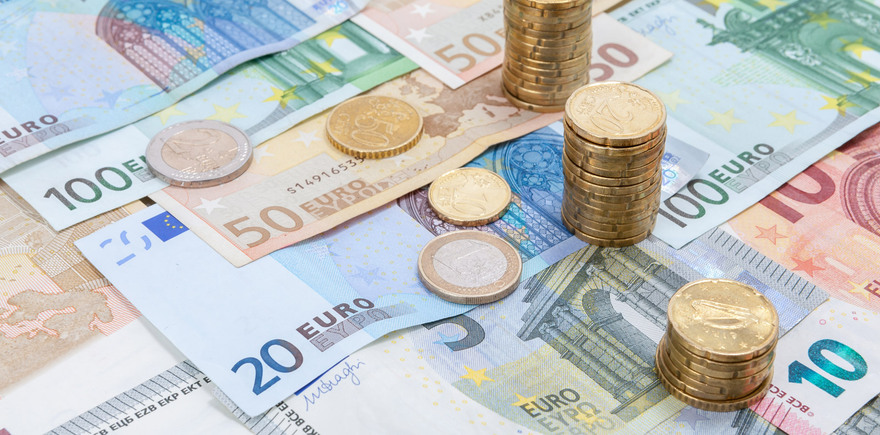
\includegraphics[max width=0.95\textwidth,
        max height=0.58000\textheight]{{Images/euro}.jpg}
    \end{center}
    \end{column}
    \end{columns}
}
\end{frame}
\begin{frame}[t]{Round 2 --- Answer Like It's 1999 --- \mbox{Answer 2}}
\vspace{-0.5em}
\begin{block}{Question}
Which word for a sensational headline designed to get online readers to follow a hyperlink was coined in 1999?
\end{block}

\visible<2->{
    \begin{columns}[T,totalwidth=\linewidth]
    \begin{column}{0.32\linewidth}
    \begin{block}{Answer}
    Clickbait
    \end{block}
    \end{column}
    \begin{column}{0.65\linewidth}
    \begin{center}
    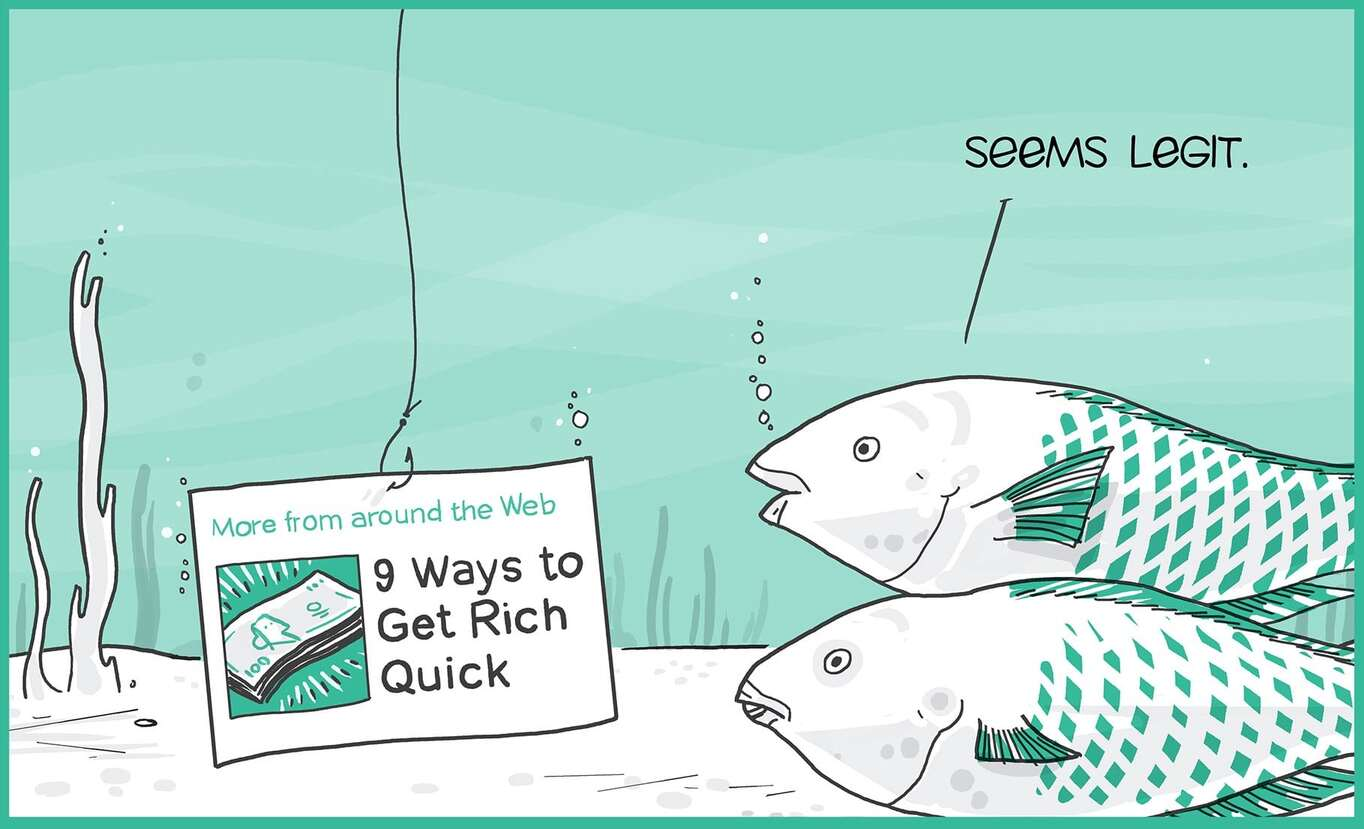
\includegraphics[max width=0.95\textwidth,
        max height=0.48000\textheight]{{Images/clickbait}.jpg}
    \end{center}
    \end{column}
    \end{columns}
}
\end{frame}
\begin{frame}[t]{Round 2 --- Answer Like It's 1999 --- \mbox{Answer 3}}
\vspace{-0.5em}
\begin{block}{Question}
On December 20, 1999, sovereignty of which former Portuguese colony was transferred to China?
\end{block}

\visible<2->{
    \begin{columns}[T,totalwidth=\linewidth]
    \begin{column}{0.32\linewidth}
    \begin{block}{Answer}
    Macau
    \end{block}
    \end{column}
    \begin{column}{0.65\linewidth}
    \begin{center}
    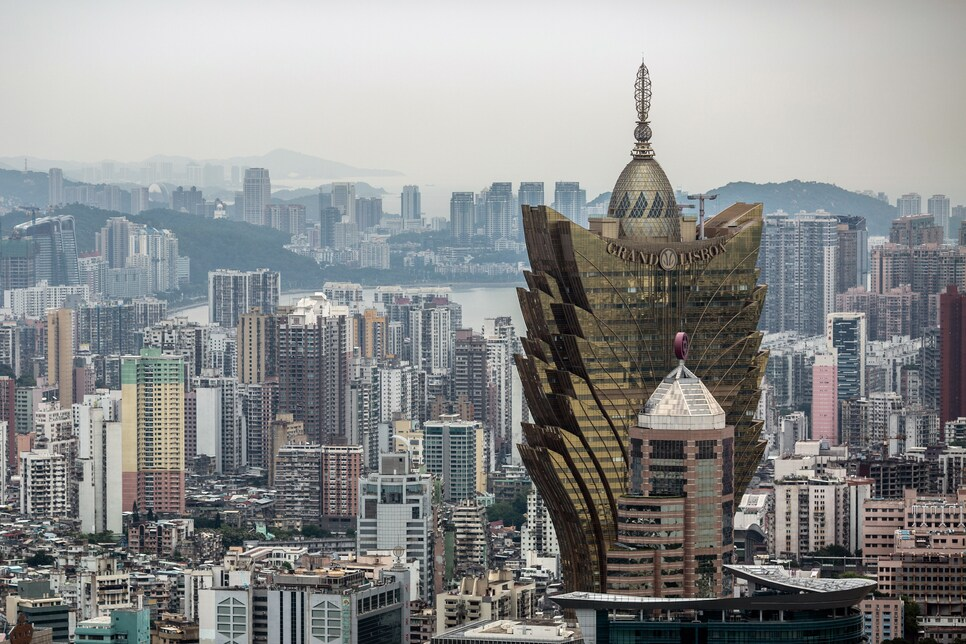
\includegraphics[max width=0.95\textwidth,
        max height=0.53000\textheight]{{Images/macau}.jpg}
    \end{center}
    \end{column}
    \end{columns}
}
\end{frame}
\begin{frame}[t]{Round 2 --- Answer Like It's 1999 --- \mbox{Answer 4}}
\vspace{-0.5em}
\begin{block}{Question}
By worldwide gross, what was the highest grossing film of 1999?
\end{block}

\visible<2->{
    \begin{columns}[T,totalwidth=\linewidth]
    \begin{column}{0.32\linewidth}
    \begin{block}{Answer}
    \emph{Star Wars: Episode I} / \emph{The Phantom Menace}
    \end{block}
    \end{column}
    \begin{column}{0.65\linewidth}
    \begin{center}
    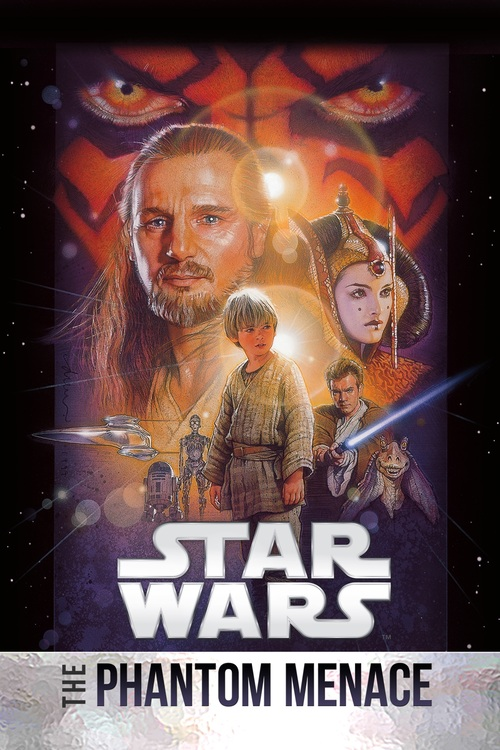
\includegraphics[max width=0.95\textwidth,
        max height=0.53000\textheight]{{Images/menace}.jpg}
    \end{center}
    \end{column}
    \end{columns}
}
\end{frame}
\begin{frame}[t]{Round 2 --- Answer Like It's 1999 --- \mbox{Answer 5}}
\vspace{-0.5em}
\begin{block}{Question}
Rapper Montero Lamar Hill, born on April 9, 1999, is better known by what stage name?
\end{block}

\visible<2->{
    \begin{columns}[T,totalwidth=\linewidth]
    \begin{column}{0.32\linewidth}
    \begin{block}{Answer}
    Lil Nas X
    \end{block}
    \end{column}
    \begin{column}{0.65\linewidth}
    \begin{center}
    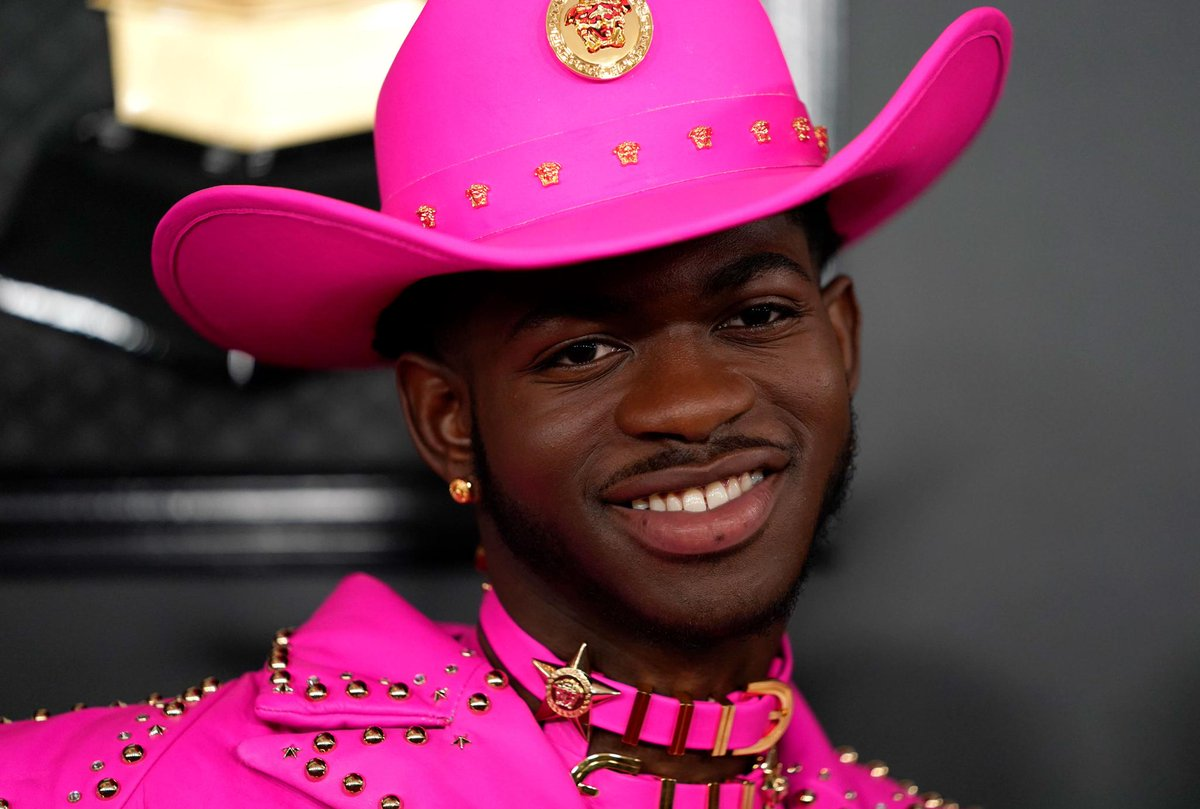
\includegraphics[max width=0.95\textwidth,
        max height=0.53000\textheight]{{Images/lilnasx}.jpg}
    \end{center}
    \end{column}
    \end{columns}
}
\end{frame}
\begin{frame}[t]{Round 2 --- Answer Like It's 1999 --- \mbox{Answer 6}}
\vspace{-0.5em}
\begin{block}{Question}
Which animated TV show that premiered in 1999 had episodes titled ``Pizza Delivery'', ``Boating School'', and ``F.U.N.''?
\end{block}

\visible<2->{
    \begin{columns}[T,totalwidth=\linewidth]
    \begin{column}{0.32\linewidth}
    \begin{block}{Answer}
    \emph{SpongeBob Squarepants} / \emph{SpongeBob}
    \end{block}
    \end{column}
    \begin{column}{0.65\linewidth}
    \begin{center}
    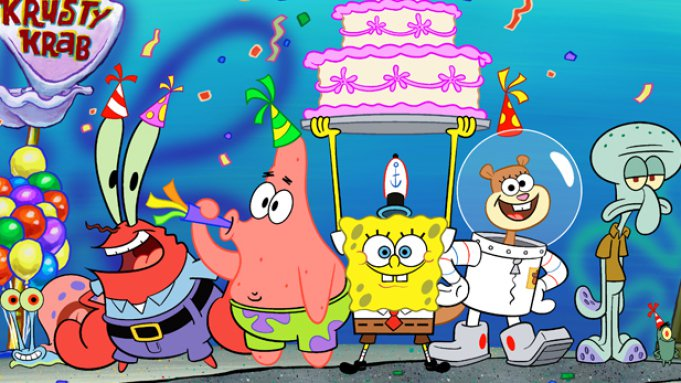
\includegraphics[max width=0.95\textwidth,
        max height=0.48000\textheight]{{Images/spongebob}.jpg}
    \end{center}
    \end{column}
    \end{columns}
}
\end{frame}
\begin{frame}[t]{Round 2 --- Answer Like It's 1999 --- \mbox{Answer 7}}
\vspace{-0.5em}
\begin{block}{Question}
Name any of the three countries that joined NATO in 1999.
\end{block}

\visible<2->{
    \begin{columns}[T,totalwidth=\linewidth]
    \begin{column}{0.32\linewidth}
    \begin{block}{Answer}
    Poland, Hungary, and the Czech Republic (you only needed one)
    \end{block}
    \end{column}
    \begin{column}{0.65\linewidth}
    \begin{center}
    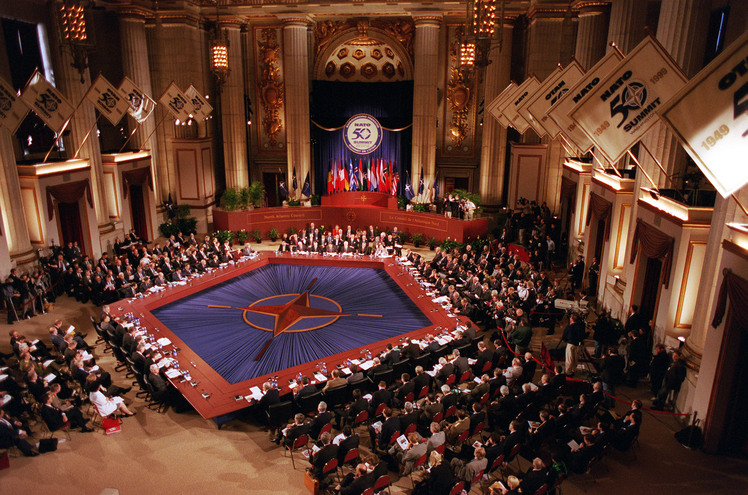
\includegraphics[max width=0.95\textwidth,
        max height=0.53000\textheight]{{Images/nato}.jpg}
    \end{center}
    \end{column}
    \end{columns}
}
\end{frame}
\begin{frame}[t]{Round 2 --- Answer Like It's 1999 --- \mbox{Answer 8}}
\vspace{-0.5em}
\begin{block}{Question}
Which band released their third studio album \emph{Millennium} on May 18, 1999?
\end{block}

\visible<2->{
    \begin{columns}[T,totalwidth=\linewidth]
    \begin{column}{0.32\linewidth}
    \begin{block}{Answer}
    The Backstreet Boys
    \end{block}
    \end{column}
    \begin{column}{0.65\linewidth}
    \begin{center}
    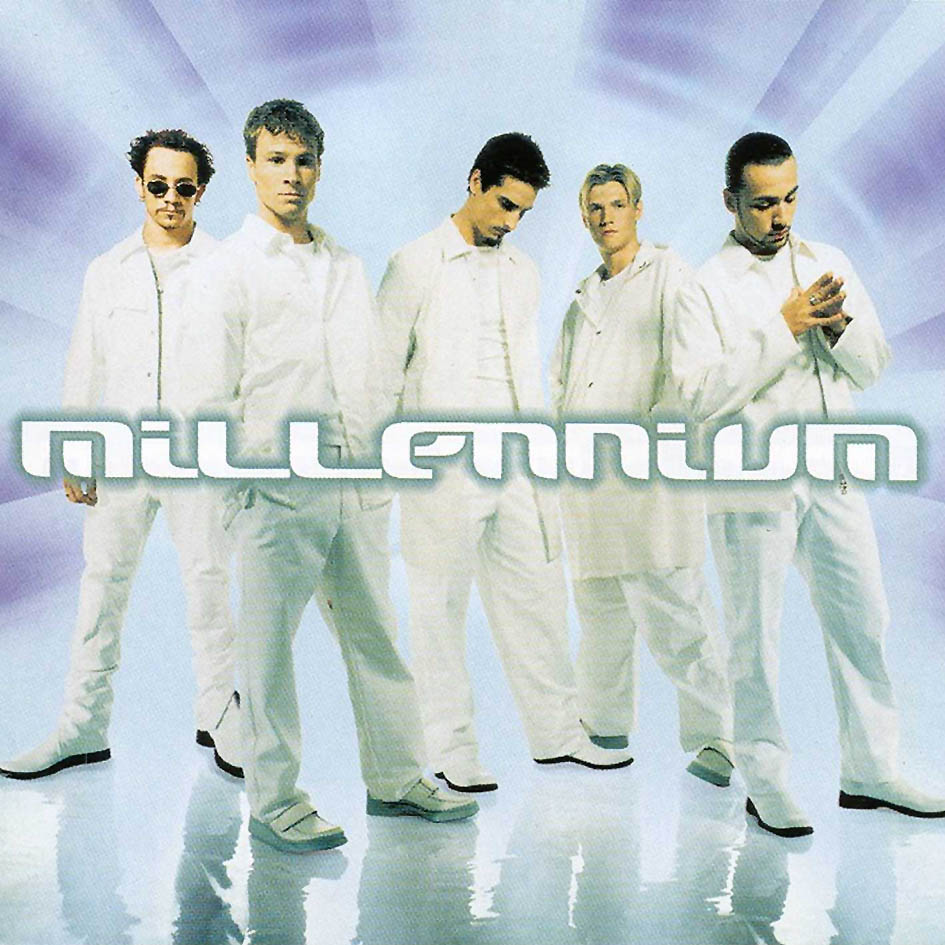
\includegraphics[max width=0.95\textwidth,
        max height=0.53000\textheight]{{Images/backstreet}.jpg}
    \end{center}
    \end{column}
    \end{columns}
}
\end{frame}
\begin{frame}[t]{Round 2 --- Answer Like It's 1999 --- \mbox{Answer 9}}
\vspace{-0.5em}
\begin{block}{Question}
On December 31, 1999, who resigned as president of Russia?
\end{block}

\visible<2->{
    \begin{columns}[T,totalwidth=\linewidth]
    \begin{column}{0.32\linewidth}
    \begin{block}{Answer}
    Boris Yeltsin
    \end{block}
    \end{column}
    \begin{column}{0.65\linewidth}
    \begin{center}
    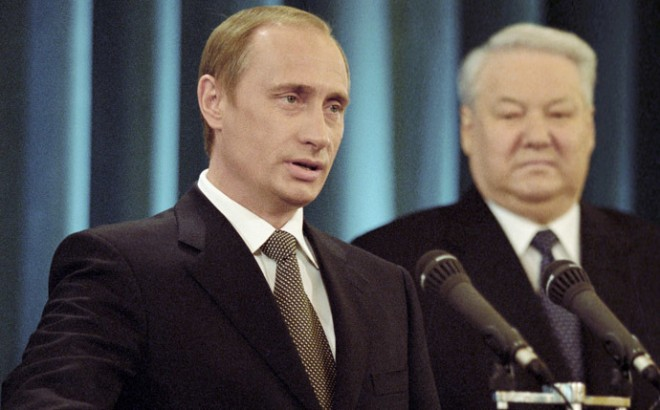
\includegraphics[max width=0.95\textwidth,
        max height=0.53000\textheight]{{Images/yeltsin}.jpg}
    \end{center}
    \end{column}
    \end{columns}
}
\end{frame}
\begin{frame}[t]{Round 2 --- Answer Like It's 1999 --- \mbox{Answer 10}}
\vspace{-0.5em}
\begin{block}{Question}
On November 30, 1999, which two large companies merged to form what was then the largest company in the world by revenue?
\end{block}

\visible<2->{
    \begin{columns}[T,totalwidth=\linewidth]
    \begin{column}{0.32\linewidth}
    \begin{block}{Answer}
    Exxon and Mobil, forming ExxonMobil
    \end{block}
    \end{column}
    \begin{column}{0.65\linewidth}
    \begin{center}
    
\includegraphics[max width=0.95\textwidth,
        max height=0.48000\textheight]{{Images/exxonmovil}.jpg}
    \end{center}
    \end{column}
    \end{columns}
}
\end{frame}
\def\thisSectionName{Count On It}
\section{Round 3}
\subsection*{Q1}
\begin{frame}[t]{Round 3 --- Count On It --- \mbox{Question 1}}
\vspace{-0.5em}
\begin{block}{Question}
To within two, how many countries are in the European Union?
\end{block}
\end{frame}
\subsection*{Q2}
\begin{frame}[t]{Round 3 --- Count On It --- \mbox{Question 2}}
\vspace{-0.5em}
\begin{block}{Question}
Not including their claws, how many legs do lobsters have?
\end{block}
\end{frame}
\subsection*{Q3}
\begin{frame}[t]{Round 3 --- Count On It --- \mbox{Question 3}}
\vspace{-0.5em}
\begin{block}{Question}
How many fluid ounces are in a gallon?
\end{block}
\end{frame}
\subsection*{Q4}
\begin{frame}[t]{Round 3 --- Count On It --- \mbox{Question 4}}
\vspace{-0.5em}
\begin{block}{Question}
How many points are there on the Statue of Liberty's crown?
\end{block}
\end{frame}
\subsection*{Q5}
\begin{frame}[t]{Round 3 --- Count On It --- \mbox{Question 5}}
\vspace{-0.5em}
\begin{block}{Question}
To within two, how many feature films (not shorts) has Pixar released? (They released two feature films in 2020.)
\end{block}
\end{frame}
\subsection*{Q6}
\begin{frame}[t]{Round 3 --- Count On It --- \mbox{Question 6}}
\vspace{-0.5em}
\begin{block}{Question}
Including wisdom teeth, how many teeth are in a full set of adult human teeth?
\end{block}
\end{frame}
\subsection*{Q7}
\begin{frame}[t]{Round 3 --- Count On It --- \mbox{Question 7}}
\vspace{-0.5em}
\begin{block}{Question}
How many stars are on the Chinese flag?
\end{block}
\end{frame}
\subsection*{Q8}
\begin{frame}[t]{Round 3 --- Count On It --- \mbox{Question 8}}
\vspace{-0.5em}
\begin{block}{Question}
How many MLB teams are there?
\end{block}
\end{frame}
\subsection*{Q9}
\begin{frame}[t]{Round 3 --- Count On It --- \mbox{Question 9}}
\vspace{-0.5em}
\begin{block}{Question}
How many people have walked on the moon?
\end{block}
\end{frame}
\subsection*{Q10}
\begin{frame}[t]{Round 3 --- Count On It --- \mbox{Question 10}}
\vspace{-0.5em}
\begin{block}{Question}
How many states were admitted to the US after 1900? (None were admitted in 1900.)
\end{block}
\end{frame}
\subsection{Answers}
\begin{frame}[t]{Round 3 --- Count On It --- \mbox{Answer 1}}
\vspace{-0.5em}
\begin{block}{Question}
To within two, how many countries are in the European Union?
\end{block}

\visible<2->{
    \begin{columns}[T,totalwidth=\linewidth]
    \begin{column}{0.32\linewidth}
    \begin{block}{Answer}
    27 (25--29 will be accepted)
    \end{block}
    \end{column}
    \begin{column}{0.65\linewidth}
    \begin{center}
    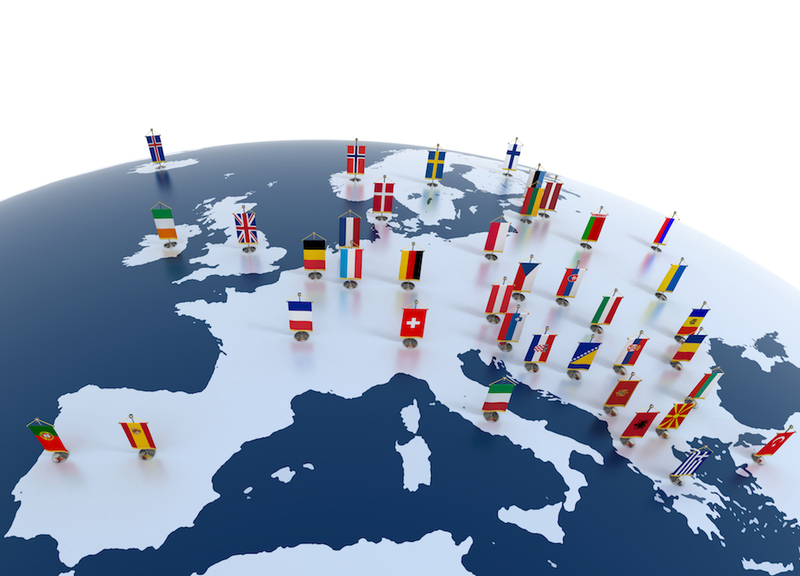
\includegraphics[max width=0.95\textwidth,
        max height=0.53000\textheight]{{Images/eu}.jpg}
    \end{center}
    \end{column}
    \end{columns}
}
\end{frame}
\begin{frame}[t]{Round 3 --- Count On It --- \mbox{Answer 2}}
\vspace{-0.5em}
\begin{block}{Question}
Not including their claws, how many legs do lobsters have?
\end{block}

\visible<2->{
    \begin{columns}[T,totalwidth=\linewidth]
    \begin{column}{0.32\linewidth}
    \begin{block}{Answer}
    Eight
    \end{block}
    \end{column}
    \begin{column}{0.65\linewidth}
    \begin{center}
    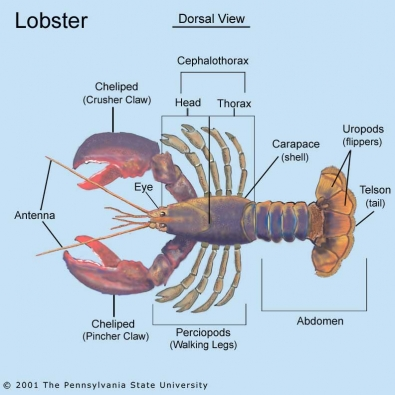
\includegraphics[max width=0.95\textwidth,
        max height=0.53000\textheight]{{Images/lobster}.jpg}
    \end{center}
    \end{column}
    \end{columns}
}
\end{frame}
\begin{frame}[t]{Round 3 --- Count On It --- \mbox{Answer 3}}
\vspace{-0.5em}
\begin{block}{Question}
How many fluid ounces are in a gallon?
\end{block}

\visible<2->{
    \begin{columns}[T,totalwidth=\linewidth]
    \begin{column}{0.32\linewidth}
    \begin{block}{Answer}
    128
    \end{block}
    \end{column}
    \begin{column}{0.65\linewidth}
    \begin{center}
    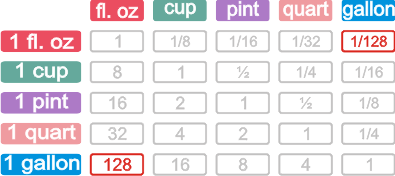
\includegraphics[max width=0.95\textwidth,
        max height=0.58000\textheight]{{Images/gallon}.png}
    \end{center}
    \end{column}
    \end{columns}
}
\end{frame}
\begin{frame}[t]{Round 3 --- Count On It --- \mbox{Answer 4}}
\vspace{-0.5em}
\begin{block}{Question}
How many points are there on the Statue of Liberty's crown?
\end{block}

\visible<2->{
    \begin{columns}[T,totalwidth=\linewidth]
    \begin{column}{0.32\linewidth}
    \begin{block}{Answer}
    Seven
    \end{block}
    \end{column}
    \begin{column}{0.65\linewidth}
    \begin{center}
    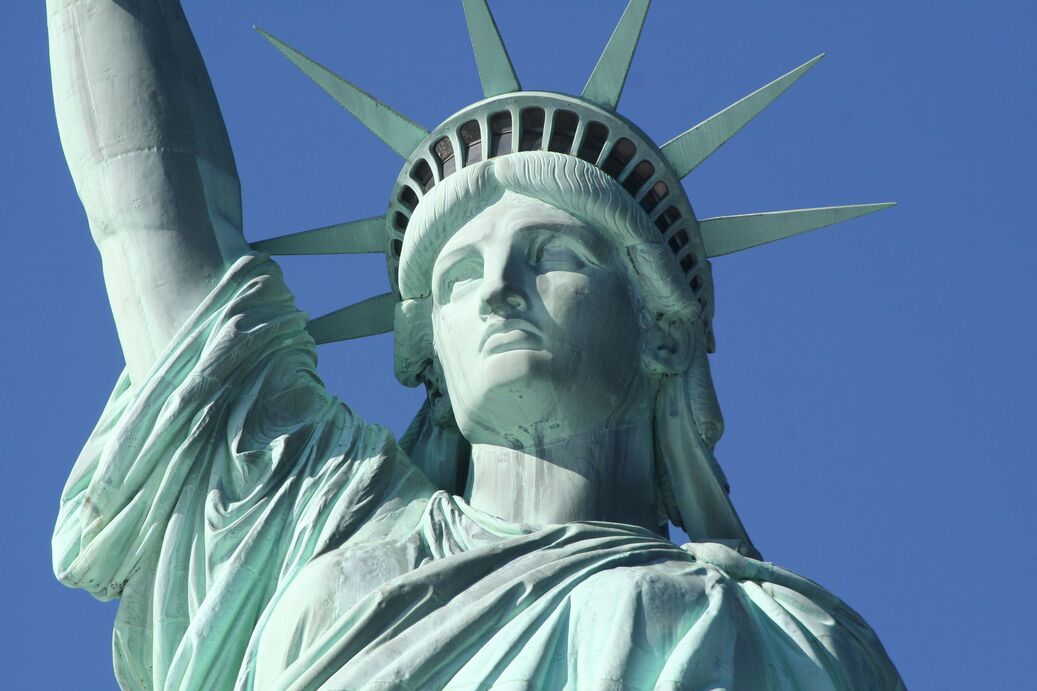
\includegraphics[max width=0.95\textwidth,
        max height=0.53000\textheight]{{Images/statueofliberty}.jpg}
    \end{center}
    \end{column}
    \end{columns}
}
\end{frame}
\begin{frame}[t]{Round 3 --- Count On It --- \mbox{Answer 5}}
\vspace{-0.5em}
\begin{block}{Question}
To within two, how many feature films (not shorts) has Pixar released? (They released two feature films in 2020.)
\end{block}

\visible<2->{
    \begin{columns}[T,totalwidth=\linewidth]
    \begin{column}{0.32\linewidth}
    \begin{block}{Answer}
    23 (21--25 will be accepted)
    \end{block}
    \end{column}
    \begin{column}{0.65\linewidth}
    \begin{center}
    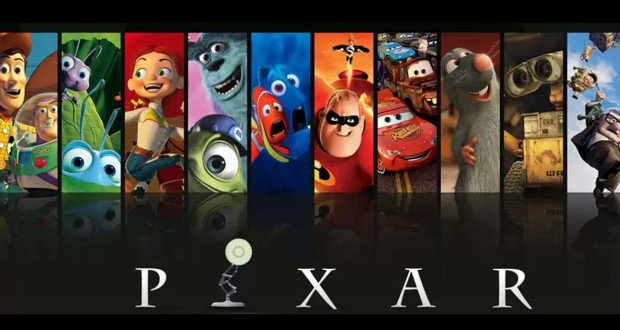
\includegraphics[max width=0.95\textwidth,
        max height=0.48000\textheight]{{Images/pixar}.jpg}
    \end{center}
    \end{column}
    \end{columns}
}
\end{frame}
\begin{frame}[t]{Round 3 --- Count On It --- \mbox{Answer 6}}
\vspace{-0.5em}
\begin{block}{Question}
Including wisdom teeth, how many teeth are in a full set of adult human teeth?
\end{block}

\visible<2->{
    \begin{columns}[T,totalwidth=\linewidth]
    \begin{column}{0.32\linewidth}
    \begin{block}{Answer}
    32
    \end{block}
    \end{column}
    \begin{column}{0.65\linewidth}
    \begin{center}
    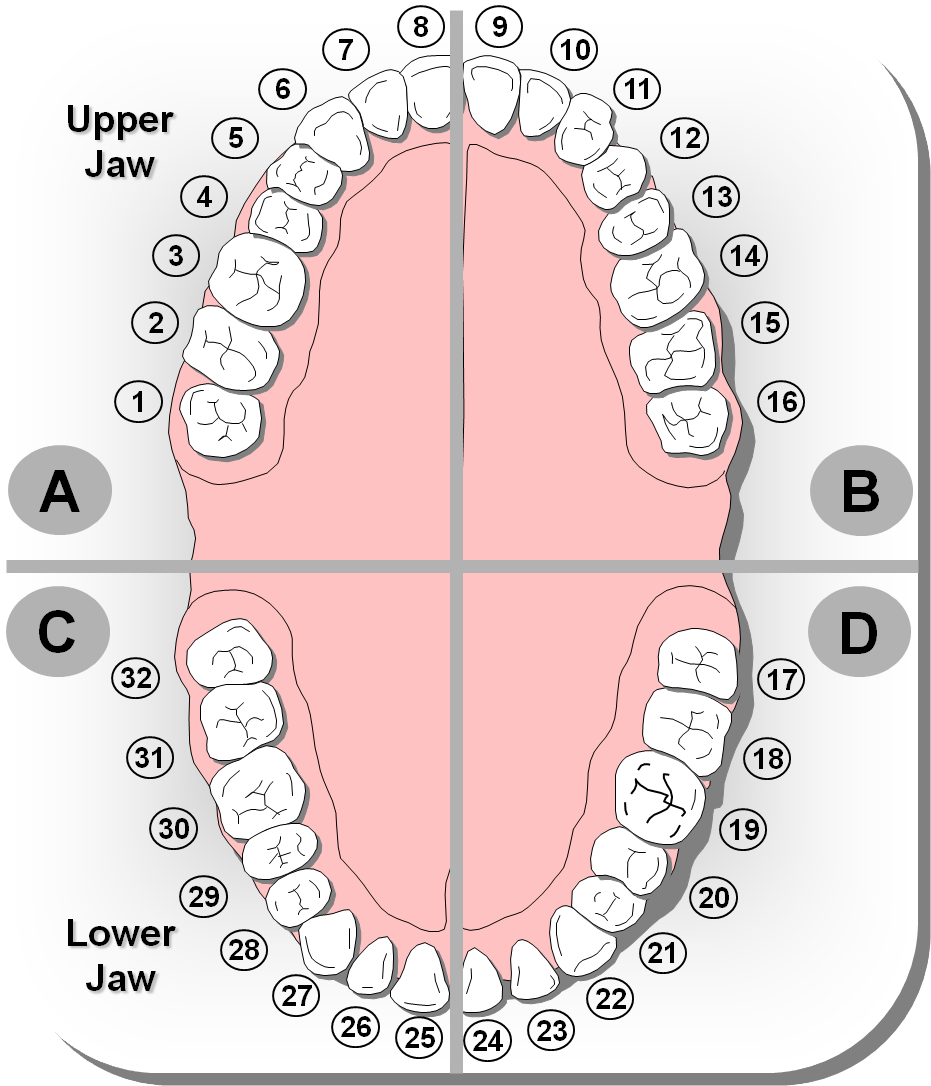
\includegraphics[max width=0.95\textwidth,
        max height=0.53000\textheight]{{Images/humanteeth}.png}
    \end{center}
    \end{column}
    \end{columns}
}
\end{frame}
\begin{frame}[t]{Round 3 --- Count On It --- \mbox{Answer 7}}
\vspace{-0.5em}
\begin{block}{Question}
How many stars are on the Chinese flag?
\end{block}

\visible<2->{
    \begin{columns}[T,totalwidth=\linewidth]
    \begin{column}{0.32\linewidth}
    \begin{block}{Answer}
    Five
    \end{block}
    \end{column}
    \begin{column}{0.65\linewidth}
    \begin{center}
    
\includegraphics[max width=0.95\textwidth,
        max height=0.58000\textheight]{{Images/chinaflag}.png}
    \end{center}
    \end{column}
    \end{columns}
}
\end{frame}
\begin{frame}[t]{Round 3 --- Count On It --- \mbox{Answer 8}}
\vspace{-0.5em}
\begin{block}{Question}
How many MLB teams are there?
\end{block}

\visible<2->{
    \begin{columns}[T,totalwidth=\linewidth]
    \begin{column}{0.32\linewidth}
    \begin{block}{Answer}
    30
    \end{block}
    \end{column}
    \begin{column}{0.65\linewidth}
    \begin{center}
    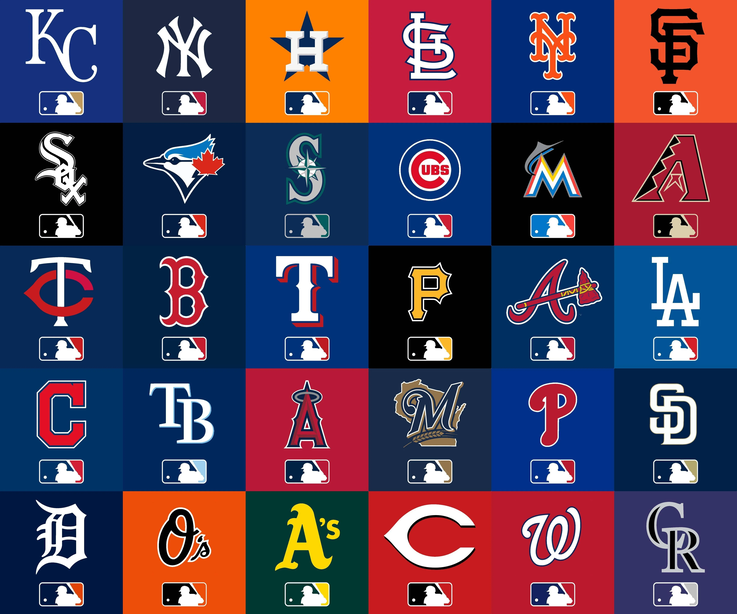
\includegraphics[max width=0.95\textwidth,
        max height=0.58000\textheight]{{Images/mlbteams}.png}
    \end{center}
    \end{column}
    \end{columns}
}
\end{frame}
\begin{frame}[t]{Round 3 --- Count On It --- \mbox{Answer 9}}
\vspace{-0.5em}
\begin{block}{Question}
How many people have walked on the moon?
\end{block}

\visible<2->{
    \begin{columns}[T,totalwidth=\linewidth]
    \begin{column}{0.32\linewidth}
    \begin{block}{Answer}
    12
    \end{block}
    \end{column}
    \begin{column}{0.65\linewidth}
    \begin{center}
    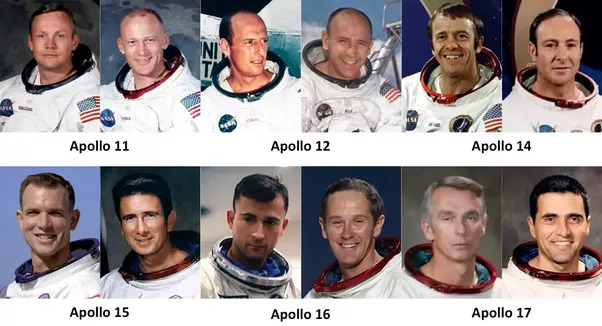
\includegraphics[max width=0.95\textwidth,
        max height=0.58000\textheight]{{Images/moonwalk}.jpg}
    \end{center}
    \end{column}
    \end{columns}
}
\end{frame}
\begin{frame}[t]{Round 3 --- Count On It --- \mbox{Answer 10}}
\vspace{-0.5em}
\begin{block}{Question}
How many states were admitted to the US after 1900? (None were admitted in 1900.)
\end{block}

\visible<2->{
    \begin{columns}[T,totalwidth=\linewidth]
    \begin{column}{0.5\linewidth}
    \begin{block}{Answer}
    Five (Oklahoma in 1907, New Mexico in 1912, Arizona in 1912, Alaska in 1959, and Hawaii in 1959)
    \end{block}
    \end{column}
    \begin{column}{0.5\linewidth}
    \begin{center}
    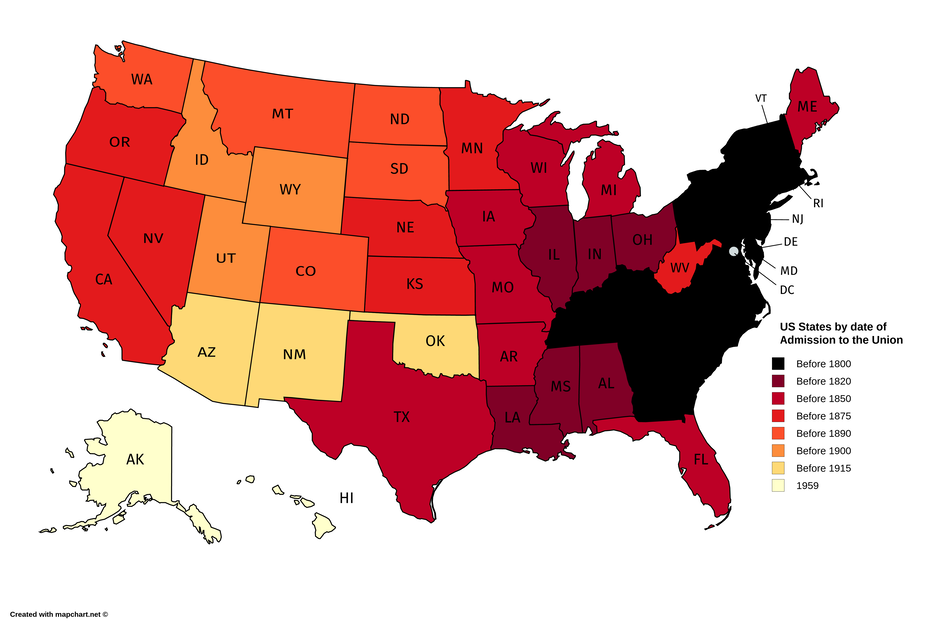
\includegraphics[max width=0.95\textwidth,
        max height=0.53000\textheight]{{Images/usstates}.png}
    \end{center}
    \end{column}
    \end{columns}
}
\end{frame}
\def\thisSectionName{Ham's Solo}
\section{Round 4}
\subsection*{Q1}
\begin{frame}[t]{Round 4 --- Ham's Solo --- \mbox{Question 1}}
\vspace{-0.5em}
\begin{block}{Question}
To be, or not to be: that is the question:\\
Whether 'tis nobler in the mind to suffer\\
The slings and arrows of outrageous \textunderscore{}\textunderscore{}\textunderscore{}\textunderscore{}\textunderscore{},
\end{block}
\end{frame}
\subsection*{Q2}
\begin{frame}[t]{Round 4 --- Ham's Solo --- \mbox{Question 2}}
\vspace{-0.5em}
\begin{block}{Question}
Or to take arms against a sea of troubles,\\
And by opposing end them? To die: to sleep;\\
No more; and by a sleep to say we end\\
The heart-ache and the thousand natural \textunderscore{}\textunderscore{}\textunderscore{}\textunderscore{}\textunderscore{}\\
That flesh is heir to\ldots{}
\end{block}
\end{frame}
\subsection*{Q3}
\begin{frame}[t]{Round 4 --- Ham's Solo --- \mbox{Question 3}}
\vspace{-0.5em}
\begin{block}{Question}
\ldots{}'tis a consummation\\
Devoutly to be wish'd. To die, to sleep;\\
To sleep: perchance to dream: ay, there's the \textunderscore{}\textunderscore{}\textunderscore{}\textunderscore{}\textunderscore{};
\end{block}
\end{frame}
\subsection*{Q4}
\begin{frame}[t]{Round 4 --- Ham's Solo --- \mbox{Question 4}}
\vspace{-0.5em}
\begin{block}{Question}
[Fill in both blanks]\\
For in that sleep of death what dreams may come\\
When we have shuffled off this \textunderscore{}\textunderscore{}\textunderscore{}\textunderscore{}\textunderscore{} \textunderscore{}\textunderscore{}\textunderscore{}\textunderscore{}\textunderscore{},\\
Must give us pause: there's the respect
\end{block}
\end{frame}
\subsection*{Q5}
\begin{frame}[t]{Round 4 --- Ham's Solo --- \mbox{Question 5}}
\vspace{-0.5em}
\begin{block}{Question}
That makes calamity of so long life;\\
For who would bear the whips and scorns of time,\\
The oppressor's wrong, the proud man's \textunderscore{}\textunderscore{}\textunderscore{}\textunderscore{}\textunderscore{},
\end{block}
\end{frame}
\subsection*{Q6}
\begin{frame}[t]{Round 4 --- Ham's Solo --- \mbox{Question 6}}
\vspace{-0.5em}
\begin{block}{Question}
The pangs of despised love, the law's delay,\\
The insolence of office and the spurns\\
That patient \textunderscore{}\textunderscore{}\textunderscore{}\textunderscore{}\textunderscore{} of the unworthy takes,
\end{block}
\end{frame}
\subsection*{Q7}
\begin{frame}[t]{Round 4 --- Ham's Solo --- \mbox{Question 7}}
\vspace{-0.5em}
\begin{block}{Question}
[Fill in both blanks]\\
When he himself might his quietus make\\
With a bare \textunderscore{}\textunderscore{}\textunderscore{}\textunderscore{}\textunderscore{}? who would \textunderscore{}\textunderscore{}\textunderscore{}\textunderscore{}\textunderscore{} bear,\\
To grunt and sweat under a weary life,
\end{block}
\end{frame}
\subsection*{Q8}
\begin{frame}[t]{Round 4 --- Ham's Solo --- \mbox{Question 8}}
\vspace{-0.5em}
\begin{block}{Question}
But that the \textunderscore{}\textunderscore{}\textunderscore{}\textunderscore{}\textunderscore{} of something after death,\\
The undiscover'd country from whose bourn\\
No traveller returns, puzzles the will
\end{block}
\end{frame}
\subsection*{Q9}
\begin{frame}[t]{Round 4 --- Ham's Solo --- \mbox{Question 9}}
\vspace{-0.5em}
\begin{block}{Question}
[Fill in both blanks]\\
And makes us rather bear those ills we have\\
Than fly to others that we know not of?\\
Thus \textunderscore{}\textunderscore{}\textunderscore{}\textunderscore{}\textunderscore{} does make \textunderscore{}\textunderscore{}\textunderscore{}\textunderscore{}\textunderscore{} of us all;
\end{block}
\end{frame}
\subsection*{Q10}
\begin{frame}[t]{Round 4 --- Ham's Solo --- \mbox{Question 10}}
\vspace{-0.5em}
\begin{block}{Question}
[Fill in two of the three blanks]\\
And thus the native \textunderscore{}\textunderscore{}\textunderscore{}\textunderscore{}\textunderscore{} of resolution\\
Is sicklied o'er with the pale \textunderscore{}\textunderscore{}\textunderscore{}\textunderscore{}\textunderscore{} of thought,\\
And enterprises of great pith and moment\\
With this regard their currents turn awry,\\
And lose the name of \textunderscore{}\textunderscore{}\textunderscore{}\textunderscore{}\textunderscore{}.---Soft you now!
\end{block}
\end{frame}
\subsection{Answers}
\begin{frame}[t]{Round 4 --- Ham's Solo --- \mbox{Answer 1}}
\vspace{-0.5em}
\begin{block}{Question}
To be, or not to be: that is the question:\\
Whether 'tis nobler in the mind to suffer\\
The slings and arrows of outrageous \textunderscore{}\textunderscore{}\textunderscore{}\textunderscore{}\textunderscore{},
\end{block}
\visible<2->{
    \begin{block}{Answer}
    Fortune
    \end{block}
}
\end{frame}
\begin{frame}[t]{Round 4 --- Ham's Solo --- \mbox{Answer 2}}
\vspace{-0.5em}
\begin{block}{Question}
Or to take arms against a sea of troubles,\\
And by opposing end them? To die: to sleep;\\
No more; and by a sleep to say we end\\
The heart-ache and the thousand natural \textunderscore{}\textunderscore{}\textunderscore{}\textunderscore{}\textunderscore{}\\
That flesh is heir to\ldots{}
\end{block}
\visible<2->{
    \begin{block}{Answer}
    Shocks
    \end{block}
}
\end{frame}
\begin{frame}[t]{Round 4 --- Ham's Solo --- \mbox{Answer 3}}
\vspace{-0.5em}
\begin{block}{Question}
\ldots{}'tis a consummation\\
Devoutly to be wish'd. To die, to sleep;\\
To sleep: perchance to dream: ay, there's the \textunderscore{}\textunderscore{}\textunderscore{}\textunderscore{}\textunderscore{};
\end{block}
\visible<2->{
    \begin{block}{Answer}
    Rub
    \end{block}
}
\end{frame}
\begin{frame}[t]{Round 4 --- Ham's Solo --- \mbox{Answer 4}}
\vspace{-0.5em}
\begin{block}{Question}
[Fill in both blanks]\\
For in that sleep of death what dreams may come\\
When we have shuffled off this \textunderscore{}\textunderscore{}\textunderscore{}\textunderscore{}\textunderscore{} \textunderscore{}\textunderscore{}\textunderscore{}\textunderscore{}\textunderscore{},\\
Must give us pause: there's the respect
\end{block}
\visible<2->{
    \begin{block}{Answer}
    Mortal coil
    \end{block}
}
\end{frame}
\begin{frame}[t]{Round 4 --- Ham's Solo --- \mbox{Answer 5}}
\vspace{-0.5em}
\begin{block}{Question}
That makes calamity of so long life;\\
For who would bear the whips and scorns of time,\\
The oppressor's wrong, the proud man's \textunderscore{}\textunderscore{}\textunderscore{}\textunderscore{}\textunderscore{},
\end{block}
\visible<2->{
    \begin{block}{Answer}
    Contumely
    \end{block}
}
\end{frame}
\begin{frame}[t]{Round 4 --- Ham's Solo --- \mbox{Answer 6}}
\vspace{-0.5em}
\begin{block}{Question}
The pangs of despised love, the law's delay,\\
The insolence of office and the spurns\\
That patient \textunderscore{}\textunderscore{}\textunderscore{}\textunderscore{}\textunderscore{} of the unworthy takes,
\end{block}
\visible<2->{
    \begin{block}{Answer}
    Merit
    \end{block}
}
\end{frame}
\begin{frame}[t]{Round 4 --- Ham's Solo --- \mbox{Answer 7}}
\vspace{-0.5em}
\begin{block}{Question}
[Fill in both blanks]\\
When he himself might his quietus make\\
With a bare \textunderscore{}\textunderscore{}\textunderscore{}\textunderscore{}\textunderscore{}? who would \textunderscore{}\textunderscore{}\textunderscore{}\textunderscore{}\textunderscore{} bear,\\
To grunt and sweat under a weary life,
\end{block}
\visible<2->{
    \begin{block}{Answer}
    Bodkin, fardels
    \end{block}
}
\end{frame}
\begin{frame}[t]{Round 4 --- Ham's Solo --- \mbox{Answer 8}}
\vspace{-0.5em}
\begin{block}{Question}
But that the \textunderscore{}\textunderscore{}\textunderscore{}\textunderscore{}\textunderscore{} of something after death,\\
The undiscover'd country from whose bourn\\
No traveller returns, puzzles the will
\end{block}
\visible<2->{
    \begin{block}{Answer}
    Dread
    \end{block}
}
\end{frame}
\begin{frame}[t]{Round 4 --- Ham's Solo --- \mbox{Answer 9}}
\vspace{-0.5em}
\begin{block}{Question}
[Fill in both blanks]\\
And makes us rather bear those ills we have\\
Than fly to others that we know not of?\\
Thus \textunderscore{}\textunderscore{}\textunderscore{}\textunderscore{}\textunderscore{} does make \textunderscore{}\textunderscore{}\textunderscore{}\textunderscore{}\textunderscore{} of us all;
\end{block}
\visible<2->{
    \begin{block}{Answer}
    Conscience, cowards
    \end{block}
}
\end{frame}
\begin{frame}[t]{Round 4 --- Ham's Solo --- \mbox{Answer 10}}
\vspace{-0.5em}
\begin{block}{Question}
[Fill in two of the three blanks]\\
And thus the native \textunderscore{}\textunderscore{}\textunderscore{}\textunderscore{}\textunderscore{} of resolution\\
Is sicklied o'er with the pale \textunderscore{}\textunderscore{}\textunderscore{}\textunderscore{}\textunderscore{} of thought,\\
And enterprises of great pith and moment\\
With this regard their currents turn awry,\\
And lose the name of \textunderscore{}\textunderscore{}\textunderscore{}\textunderscore{}\textunderscore{}.---Soft you now!
\end{block}
\visible<2->{
    \begin{block}{Answer}
    Hue, cast, action (we only needed two)
    \end{block}
}
\end{frame}
\def\thisSectionName{Philosophy and Philosophers}
\section{Round 5}
\subsection*{Q1}
\begin{frame}[t]{Round 5 --- Philosophy and Philosophers --- \mbox{Question 1}}
\vspace{-0.5em}
\begin{block}{Question}
Fill in the blanks: In Greek, ``philosophy'' literally means the \textunderscore{}\textunderscore{}\textunderscore{}\textunderscore{}\textunderscore{} of \textunderscore{}\textunderscore{}\textunderscore{}\textunderscore{}\textunderscore{}.
\end{block}
\end{frame}
\subsection*{Q2}
\begin{frame}[t]{Round 5 --- Philosophy and Philosophers --- \mbox{Question 2}}
\vspace{-0.5em}
\begin{block}{Question}
What is the title of the collection of teachings of Confucius?
\end{block}
\end{frame}
\subsection*{Q3}
\begin{frame}[t]{Round 5 --- Philosophy and Philosophers --- \mbox{Question 3}}
\vspace{-0.5em}
\begin{block}{Question}
Put these Ancient Greek philosophers in order from earliest to most recent: Aristotle, Plato, Pythagoras, and Socrates.
\end{block}
\end{frame}
\subsection*{Q4}
\begin{frame}[t]{Round 5 --- Philosophy and Philosophers --- \mbox{Question 4}}
\vspace{-0.5em}
\begin{block}{Question}
What is the name of the  philosopher who wrote \emph{Leviathan}?
\end{block}
\end{frame}
\subsection*{Q5}
\begin{frame}[t]{Round 5 --- Philosophy and Philosophers --- \mbox{Question 5}}
\vspace{-0.5em}
\begin{block}{Question}
Name either of the two Ancient Greek philosophers --- one a teacher and the other his pupil --- credited with first proposing the atomic theory, which states that matter is made of indivisible particles.
\end{block}
\end{frame}
\subsection*{Q6}
\begin{frame}[t]{Round 5 --- Philosophy and Philosophers --- \mbox{Question 6}}
\vspace{-0.5em}
\begin{block}{Question}
What is the name of the philosophical system developed by Ayn Rand?
\end{block}
\end{frame}
\subsection*{Q7}
\begin{frame}[t]{Round 5 --- Philosophy and Philosophers --- \mbox{Question 7}}
\vspace{-0.5em}
\begin{block}{Question}
Who is famous for having said ``God is dead. God remains dead. And we have killed him.''?
\end{block}
\end{frame}
\subsection*{Q8}
\begin{frame}[t]{Round 5 --- Philosophy and Philosophers --- \mbox{Question 8}}
\vspace{-0.5em}
\begin{block}{Question}
What is the name of the philosophy that posits that the only thing whose existence one can be sure of is one's own mind?
\end{block}
\end{frame}
\subsection*{Q9}
\begin{frame}[t]{Round 5 --- Philosophy and Philosophers --- \mbox{Question 9}}
\vspace{-0.5em}
\begin{block}{Question}
Which philosopher founded the doctrine of ``transcendental idealism'', which posits that only our observations of reality, but not reality itself, are cognizable?
\end{block}
\end{frame}
\subsection*{Q10}
\begin{frame}[t]{Round 5 --- Philosophy and Philosophers --- \mbox{Question 10}}
\vspace{-0.5em}
\begin{block}{Question}
Which 19\textsuperscript{th} Century American philosopher was a leader of the transcendentalist movement and championed individualism?
\end{block}
\end{frame}
\subsection{Answers}
\begin{frame}[t]{Round 5 --- Philosophy and Philosophers --- \mbox{Answer 1}}
\vspace{-0.5em}
\begin{block}{Question}
Fill in the blanks: In Greek, ``philosophy'' literally means the \textunderscore{}\textunderscore{}\textunderscore{}\textunderscore{}\textunderscore{} of \textunderscore{}\textunderscore{}\textunderscore{}\textunderscore{}\textunderscore{}.
\end{block}

\visible<2->{
    \begin{columns}[T,totalwidth=\linewidth]
    \begin{column}{0.32\linewidth}
    \begin{block}{Answer}
    The love of knowledge / wisdom
    \end{block}
    \end{column}
    \begin{column}{0.65\linewidth}
    \begin{center}
    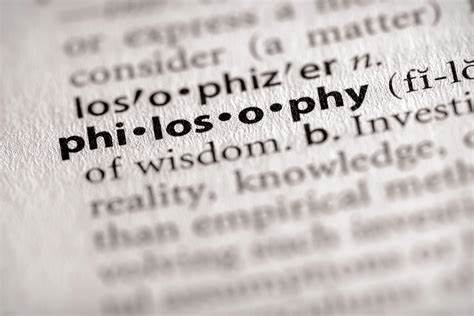
\includegraphics[max width=0.95\textwidth,
        max height=0.38000\textheight]{{Images/philosophy}.jpeg}
    \end{center}
    \end{column}
    \end{columns}
}
\end{frame}
\begin{frame}[t]{Round 5 --- Philosophy and Philosophers --- \mbox{Answer 2}}
\vspace{-0.5em}
\begin{block}{Question}
What is the title of the collection of teachings of Confucius?
\end{block}

\visible<2->{
    \begin{columns}[T,totalwidth=\linewidth]
    \begin{column}{0.32\linewidth}
    \begin{block}{Answer}
    The \emph{Analects}
    \end{block}
    \end{column}
    \begin{column}{0.65\linewidth}
    \begin{center}
    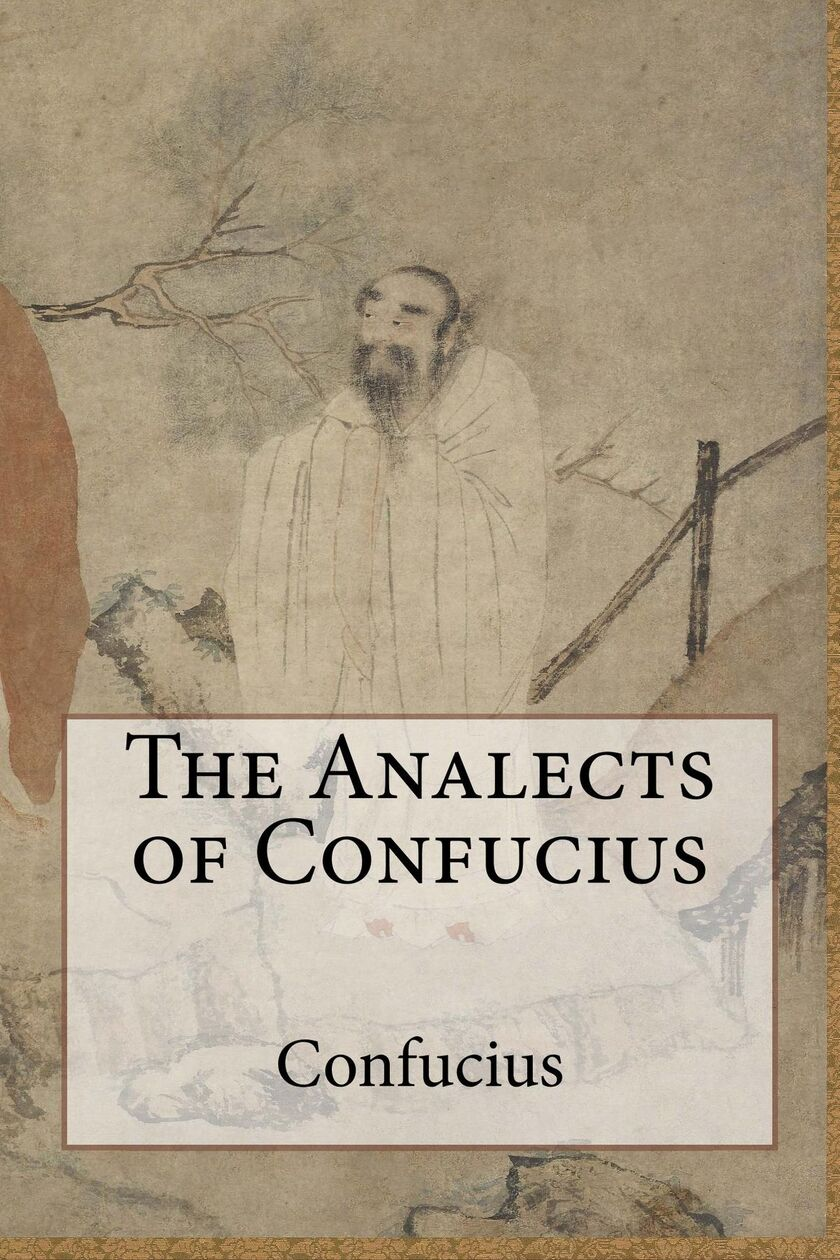
\includegraphics[max width=0.95\textwidth,
        max height=0.53000\textheight]{{Images/analects}.jpg}
    \end{center}
    \end{column}
    \end{columns}
}
\end{frame}
\begin{frame}[t]{Round 5 --- Philosophy and Philosophers --- \mbox{Answer 3}}
\vspace{-0.5em}
\begin{block}{Question}
Put these Ancient Greek philosophers in order from earliest to most recent: Aristotle, Plato, Pythagoras, and Socrates.
\end{block}

\visible<2->{
    \begin{columns}[T,totalwidth=\linewidth]
    \begin{column}{0.32\linewidth}
    \begin{block}{Answer}
    Pythagoras, Socrates, Plato, Aristotle
    \end{block}
    \end{column}
    \begin{column}{0.65\linewidth}
    \begin{center}
    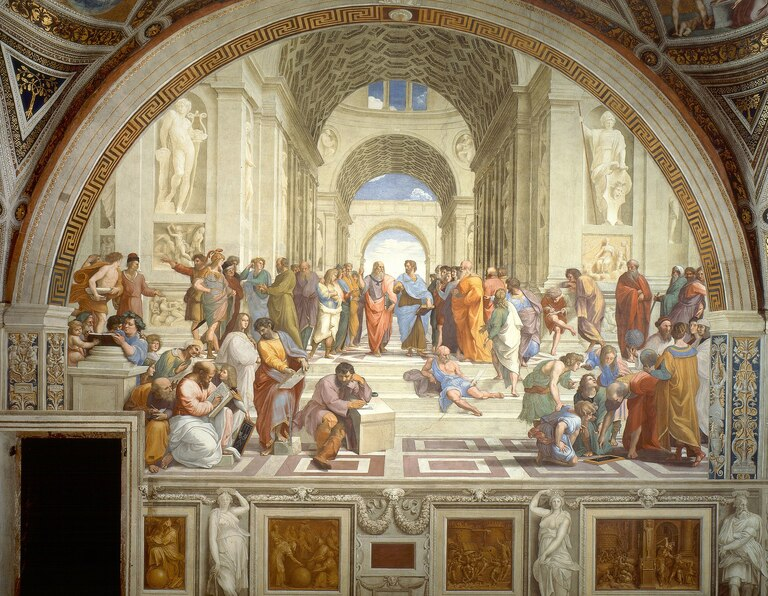
\includegraphics[max width=0.95\textwidth,
        max height=0.48000\textheight]{{Images/greeks}.jpg}
    \end{center}
    \end{column}
    \end{columns}
}
\end{frame}
\begin{frame}[t]{Round 5 --- Philosophy and Philosophers --- \mbox{Answer 4}}
\vspace{-0.5em}
\begin{block}{Question}
What is the name of the  philosopher who wrote \emph{Leviathan}?
\end{block}

\visible<2->{
    \begin{columns}[T,totalwidth=\linewidth]
    \begin{column}{0.32\linewidth}
    \begin{block}{Answer}
    Thomas Hobbes
    \end{block}
    \end{column}
    \begin{column}{0.65\linewidth}
    \begin{center}
    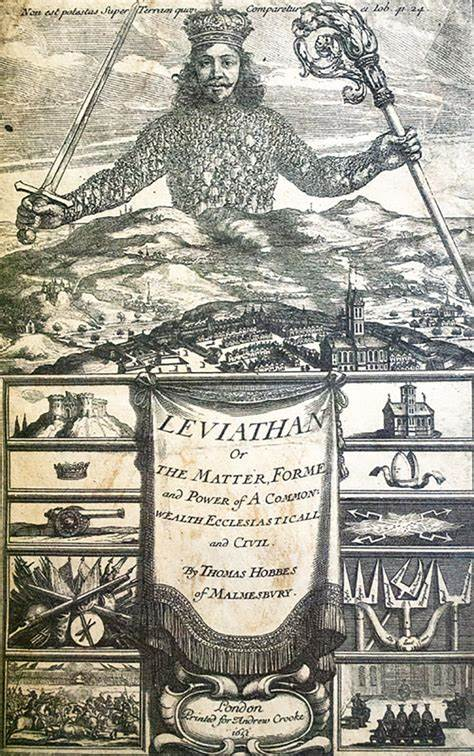
\includegraphics[max width=0.95\textwidth,
        max height=0.53000\textheight]{{Images/leviathan}.jpeg}
    \end{center}
    \end{column}
    \end{columns}
}
\end{frame}
\begin{frame}[t]{Round 5 --- Philosophy and Philosophers --- \mbox{Answer 5}}
\vspace{-0.5em}
\begin{block}{Question}
Name either of the two Ancient Greek philosophers --- one a teacher and the other his pupil --- credited with first proposing the atomic theory, which states that matter is made of indivisible particles.
\end{block}

\visible<2->{
    \begin{columns}[T,totalwidth=\linewidth]
    \begin{column}{0.32\linewidth}
    \begin{block}{Answer}
    Leucippus (teacher) and Democritus (his pupil) (we only needed one)
    \end{block}
    \end{column}
    \begin{column}{0.65\linewidth}
    \begin{center}
    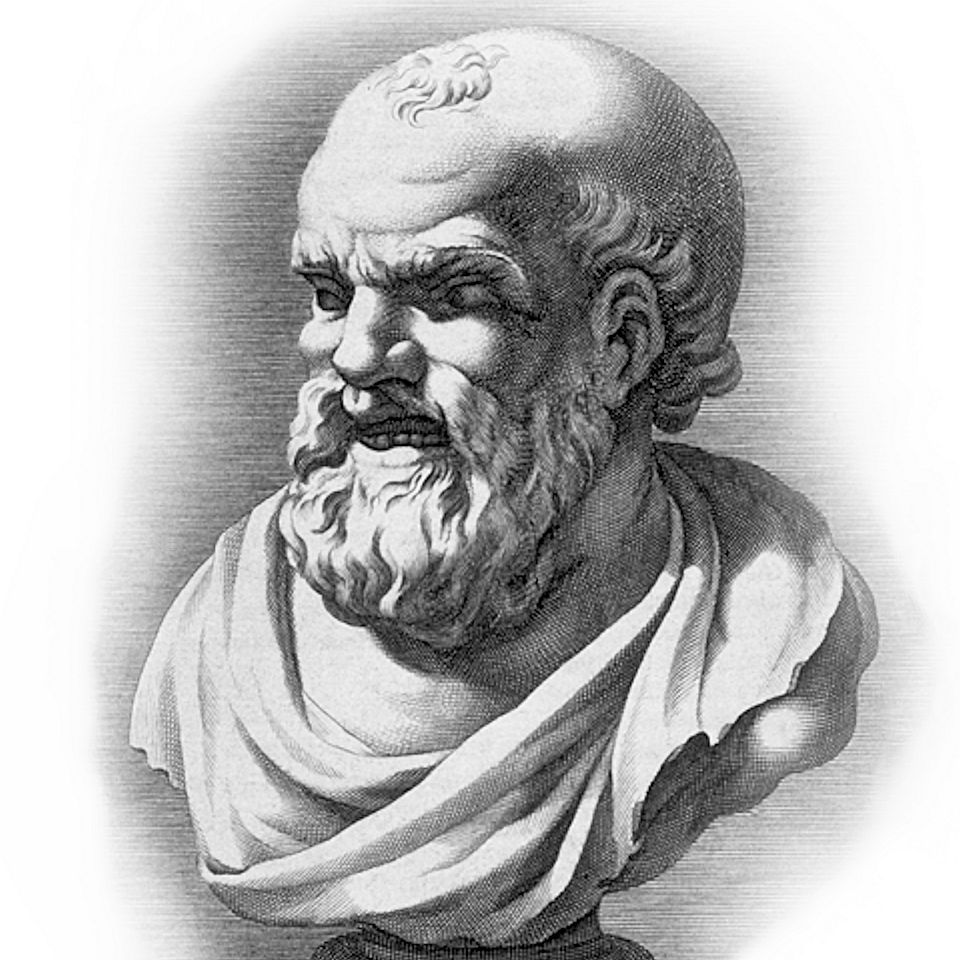
\includegraphics[max width=0.95\textwidth,
        max height=0.38000\textheight]{{Images/democritus}.jpg}
    \end{center}
    \end{column}
    \end{columns}
}
\end{frame}
\begin{frame}[t]{Round 5 --- Philosophy and Philosophers --- \mbox{Answer 6}}
\vspace{-0.5em}
\begin{block}{Question}
What is the name of the philosophical system developed by Ayn Rand?
\end{block}

\visible<2->{
    \begin{columns}[T,totalwidth=\linewidth]
    \begin{column}{0.32\linewidth}
    \begin{block}{Answer}
    Objectivisim
    \end{block}
    \end{column}
    \begin{column}{0.65\linewidth}
    \begin{center}
    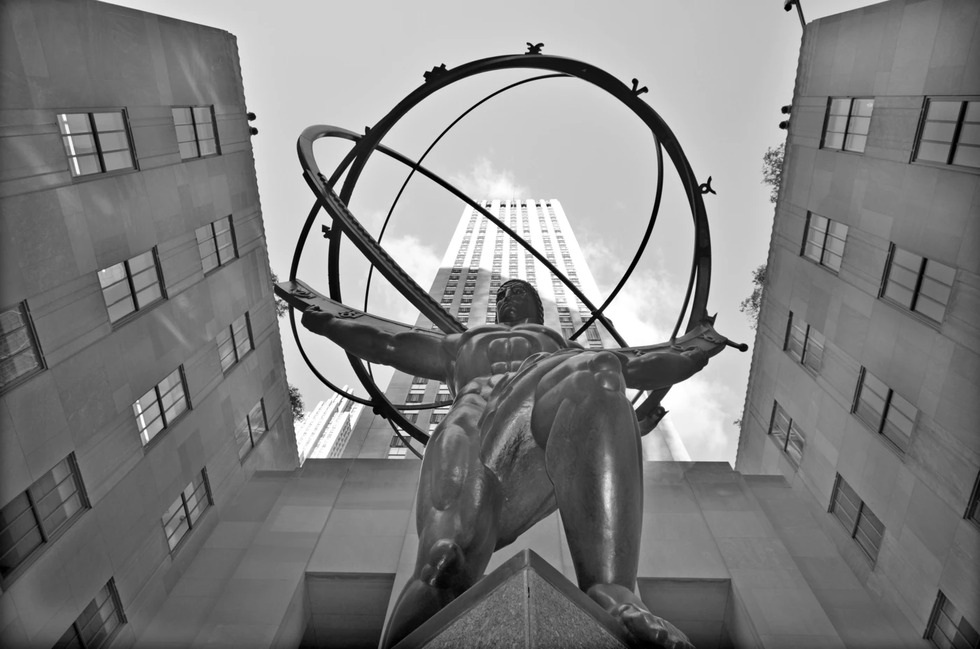
\includegraphics[max width=0.95\textwidth,
        max height=0.53000\textheight]{{Images/atlas}.jpg}
    \end{center}
    \end{column}
    \end{columns}
}
\end{frame}
\begin{frame}[t]{Round 5 --- Philosophy and Philosophers --- \mbox{Answer 7}}
\vspace{-0.5em}
\begin{block}{Question}
Who is famous for having said ``God is dead. God remains dead. And we have killed him.''?
\end{block}

\visible<2->{
    \begin{columns}[T,totalwidth=\linewidth]
    \begin{column}{0.32\linewidth}
    \begin{block}{Answer}
    Friedrich Nietzsche
    \end{block}
    \end{column}
    \begin{column}{0.65\linewidth}
    \begin{center}
    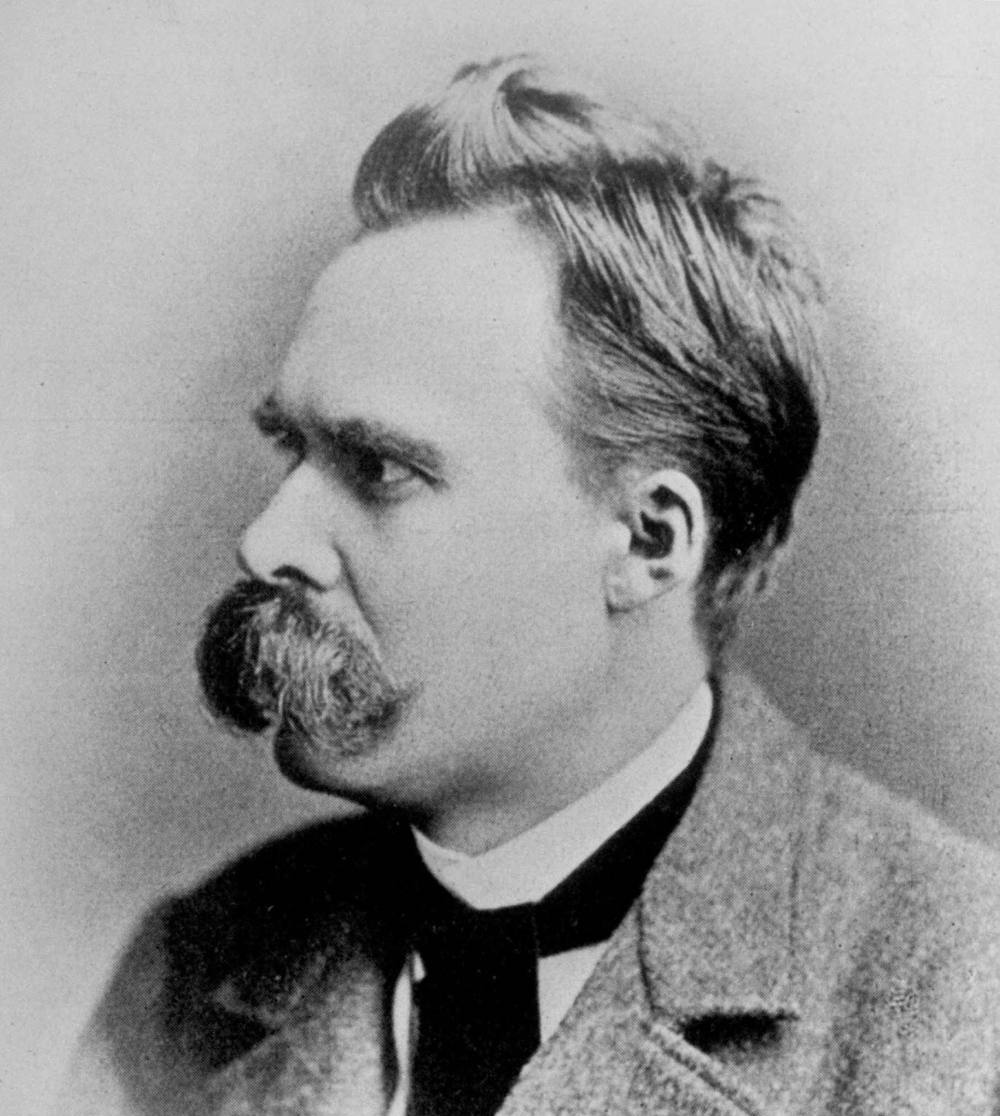
\includegraphics[max width=0.95\textwidth,
        max height=0.53000\textheight]{{Images/nietzsche}.jpg}
    \end{center}
    \end{column}
    \end{columns}
}
\end{frame}
\begin{frame}[t]{Round 5 --- Philosophy and Philosophers --- \mbox{Answer 8}}
\vspace{-0.5em}
\begin{block}{Question}
What is the name of the philosophy that posits that the only thing whose existence one can be sure of is one's own mind?
\end{block}

\visible<2->{
    \begin{columns}[T,totalwidth=\linewidth]
    \begin{column}{0.32\linewidth}
    \begin{block}{Answer}
    Solipsism
    \end{block}
    \end{column}
    \begin{column}{0.65\linewidth}
    \begin{center}
    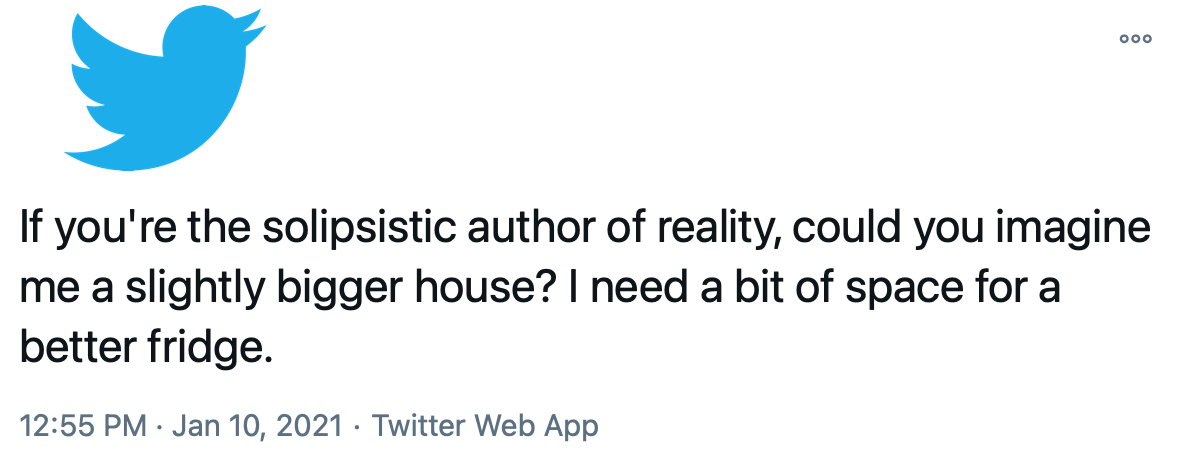
\includegraphics[max width=0.95\textwidth,
        max height=0.48000\textheight]{{Images/solipsism}.png}
    \end{center}
    \end{column}
    \end{columns}
}
\end{frame}
\begin{frame}[t]{Round 5 --- Philosophy and Philosophers --- \mbox{Answer 9}}
\vspace{-0.5em}
\begin{block}{Question}
Which philosopher founded the doctrine of ``transcendental idealism'', which posits that only our observations of reality, but not reality itself, are cognizable?
\end{block}

\visible<2->{
    \begin{columns}[T,totalwidth=\linewidth]
    \begin{column}{0.32\linewidth}
    \begin{block}{Answer}
    Immanuel Kant
    \end{block}
    \end{column}
    \begin{column}{0.65\linewidth}
    \begin{center}
    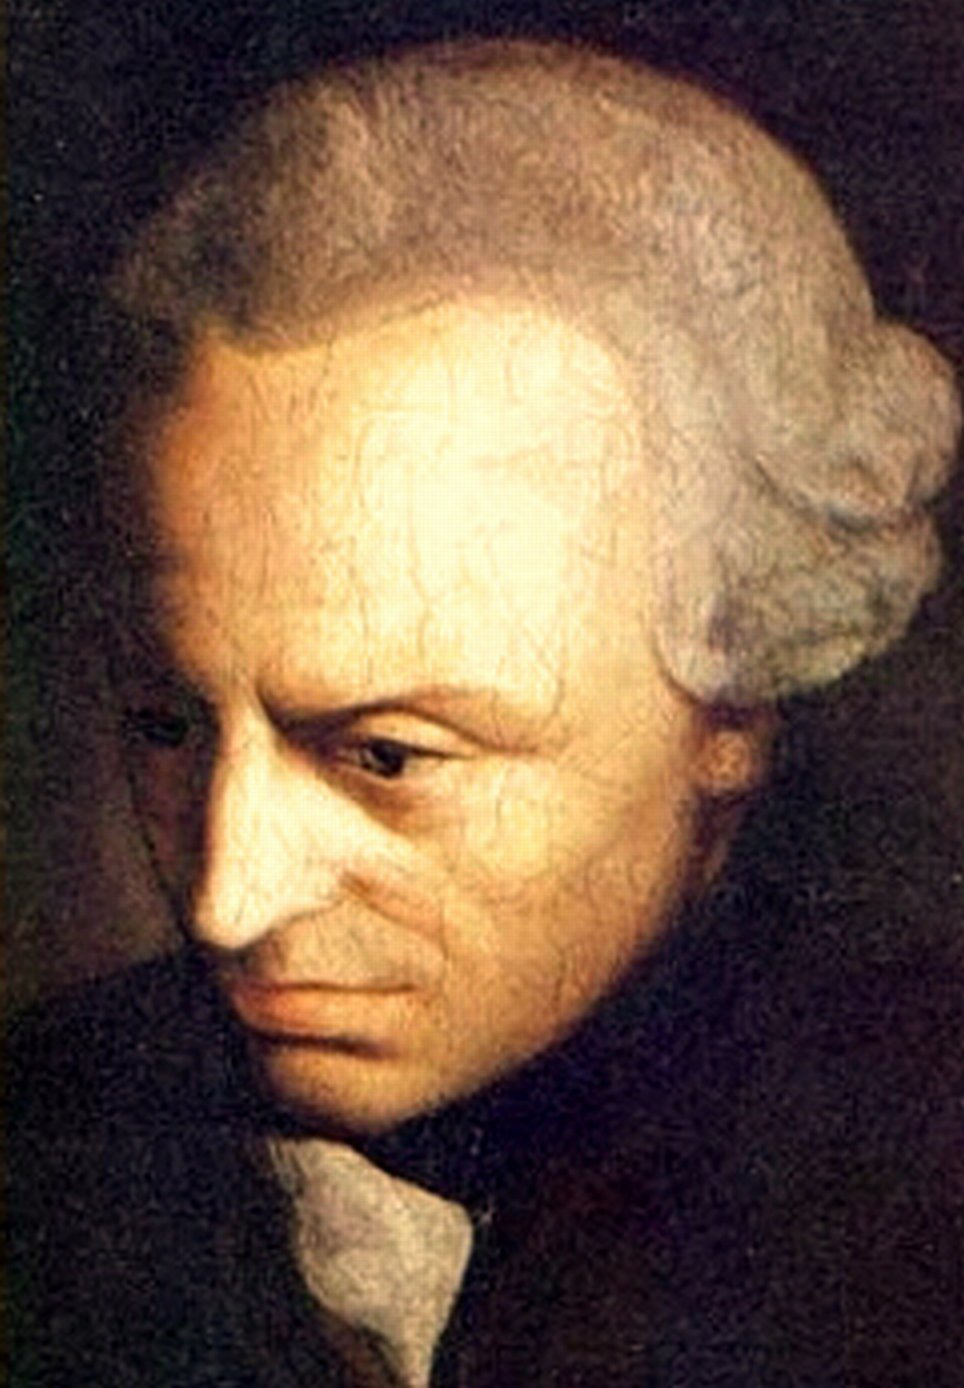
\includegraphics[max width=0.95\textwidth,
        max height=0.43000\textheight]{{Images/kant}.jpg}
    \end{center}
    \end{column}
    \end{columns}
}
\end{frame}
\begin{frame}[t]{Round 5 --- Philosophy and Philosophers --- \mbox{Answer 10}}
\vspace{-0.5em}
\begin{block}{Question}
Which 19\textsuperscript{th} Century American philosopher was a leader of the transcendentalist movement and championed individualism?
\end{block}

\visible<2->{
    \begin{columns}[T,totalwidth=\linewidth]
    \begin{column}{0.32\linewidth}
    \begin{block}{Answer}
    Ralph Waldo Emerson
    \end{block}
    \end{column}
    \begin{column}{0.65\linewidth}
    \begin{center}
    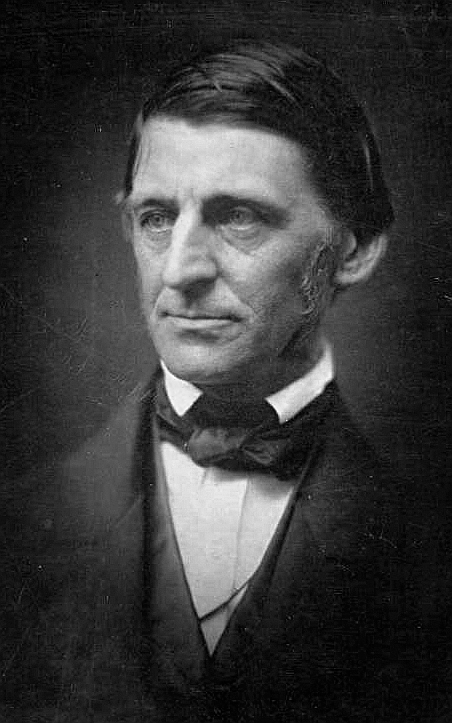
\includegraphics[max width=0.95\textwidth,
        max height=0.48000\textheight]{{Images/emerson}.jpg}
    \end{center}
    \end{column}
    \end{columns}
}
\end{frame}
\def\thisSectionName{Planet Earth}
\section{Round 6}
\subsection*{Q1}
\begin{frame}[t]{Round 6 --- Planet Earth --- \mbox{Question 1}}
\vspace{-0.5em}
\begin{block}{Question}
To within half a billion years, how old is planet Earth? In other words, how long ago did most of the material that formed the Earth gather into a sphere?
\end{block}
\end{frame}
\subsection*{Q2}
\begin{frame}[t]{Round 6 --- Planet Earth --- \mbox{Question 2}}
\vspace{-0.5em}
\begin{block}{Question}
What is the technical term for the process by which life arises from non-living materials, which occurred on Earth roughly 4 billion years ago?
\end{block}
\end{frame}
\subsection*{Q3}
\begin{frame}[t]{Round 6 --- Planet Earth --- \mbox{Question 3}}
\vspace{-0.5em}
\begin{block}{Question}
The ``Great Oxidation Event'' began roughly 2 billion years ago when atmospheric oxygen was produced as a waste product of what biological process?
\end{block}
\end{frame}
\subsection*{Q4}
\begin{frame}[t]{Round 6 --- Planet Earth --- \mbox{Question 4}}
\vspace{-0.5em}
\begin{block}{Question}
The radioactive dating method used to determine the age of the oldest rocks on Earth uses the ratio of which two elements to determine the age of a rock?
\end{block}
\end{frame}
\subsection*{Q5}
\begin{frame}[t]{Round 6 --- Planet Earth --- \mbox{Question 5}}
\vspace{-0.5em}
\begin{block}{Question}
Which layer of the atmosphere is responsible for absorbing much of the Sun's ultraviolet radiation?
\end{block}
\end{frame}
\subsection*{Q6}
\begin{frame}[t]{Round 6 --- Planet Earth --- \mbox{Question 6}}
\vspace{-0.5em}
\begin{block}{Question}
What was the name of the supercontinent that existed from roughly 300 million years ago to 180 million years ago?
\end{block}
\end{frame}
\subsection*{Q7}
\begin{frame}[t]{Round 6 --- Planet Earth --- \mbox{Question 7}}
\vspace{-0.5em}
\begin{block}{Question}
What was the ``Chicxulub impactor'', which formed the Chicxulub crater in the Yucatan Peninsula?
\end{block}
\end{frame}
\subsection*{Q8}
\begin{frame}[t]{Round 6 --- Planet Earth --- \mbox{Question 8}}
\vspace{-0.5em}
\begin{block}{Question}
The dynamo theory proposes a mechanism by which molten metal in the Earth's center can produce what?
\end{block}
\end{frame}
\subsection*{Q9}
\begin{frame}[t]{Round 6 --- Planet Earth --- \mbox{Question 9}}
\vspace{-0.5em}
\begin{block}{Question}
The stream of charged particles released from the Sun out into the solar system, known as solar wind, causes what night-sky natural phenomenon on Earth?
\end{block}
\end{frame}
\subsection*{Q10}
\begin{frame}[t]{Round 6 --- Planet Earth --- \mbox{Question 10}}
\vspace{-0.5em}
\begin{block}{Question}
What is the defining feature of the two lines of latitude known as the Tropic of Cancer and the Tropic of Capricorn?
\end{block}
\end{frame}
\subsection{Answers}
\begin{frame}[t]{Round 6 --- Planet Earth --- \mbox{Answer 1}}
\vspace{-0.5em}
\begin{block}{Question}
To within half a billion years, how old is planet Earth? In other words, how long ago did most of the material that formed the Earth gather into a sphere?
\end{block}

\visible<2->{
    \begin{columns}[T,totalwidth=\linewidth]
    \begin{column}{0.32\linewidth}
    \begin{block}{Answer}
    4.5 billion years (4--5 billion years will be accepted)
    \end{block}
    \end{column}
    \begin{column}{0.65\linewidth}
    \begin{center}
    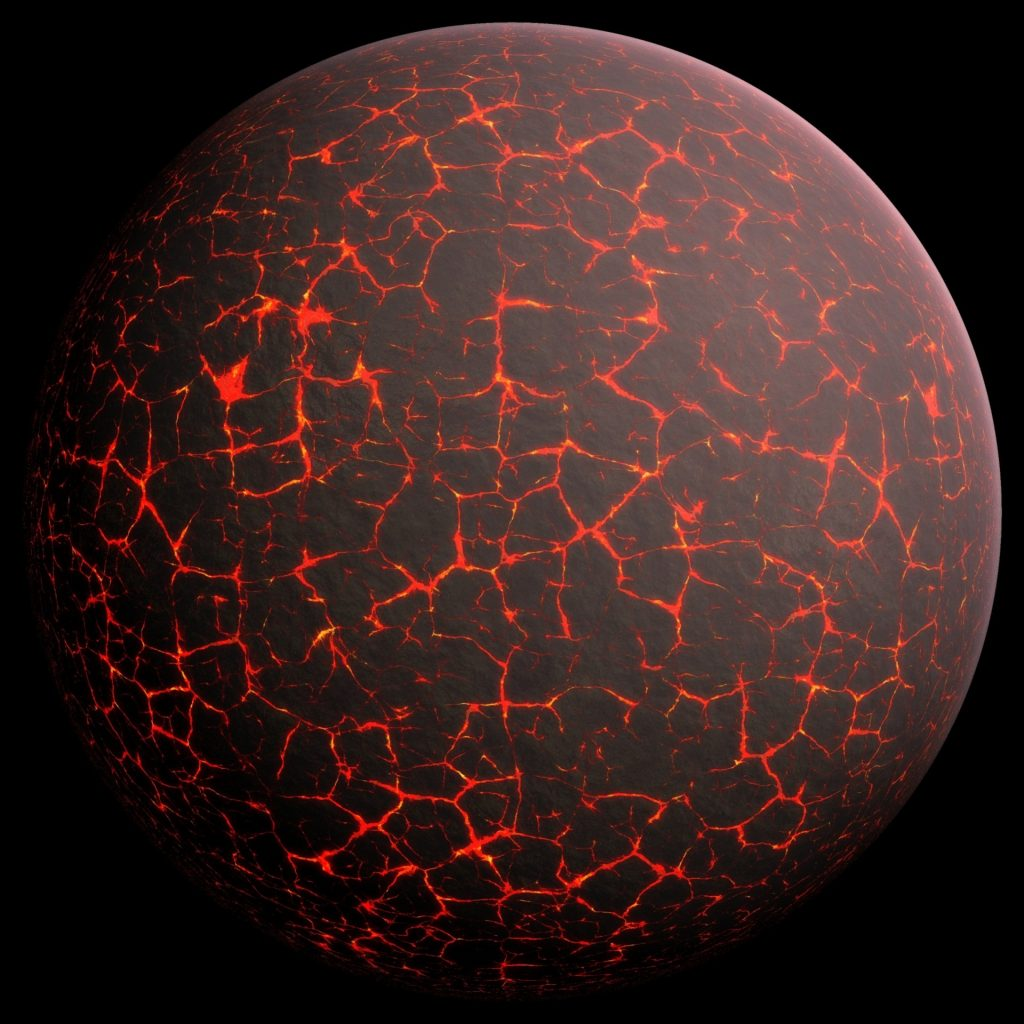
\includegraphics[max width=0.95\textwidth,
        max height=0.43000\textheight]{{Images/earthold}.jpg}
    \end{center}
    \end{column}
    \end{columns}
}
\end{frame}
\begin{frame}[t]{Round 6 --- Planet Earth --- \mbox{Answer 2}}
\vspace{-0.5em}
\begin{block}{Question}
What is the technical term for the process by which life arises from non-living materials, which occurred on Earth roughly 4 billion years ago?
\end{block}

\visible<2->{
    \begin{columns}[T,totalwidth=\linewidth]
    \begin{column}{0.32\linewidth}
    \begin{block}{Answer}
    Abiogenesis
    \end{block}
    \end{column}
    \begin{column}{0.65\linewidth}
    \begin{center}
    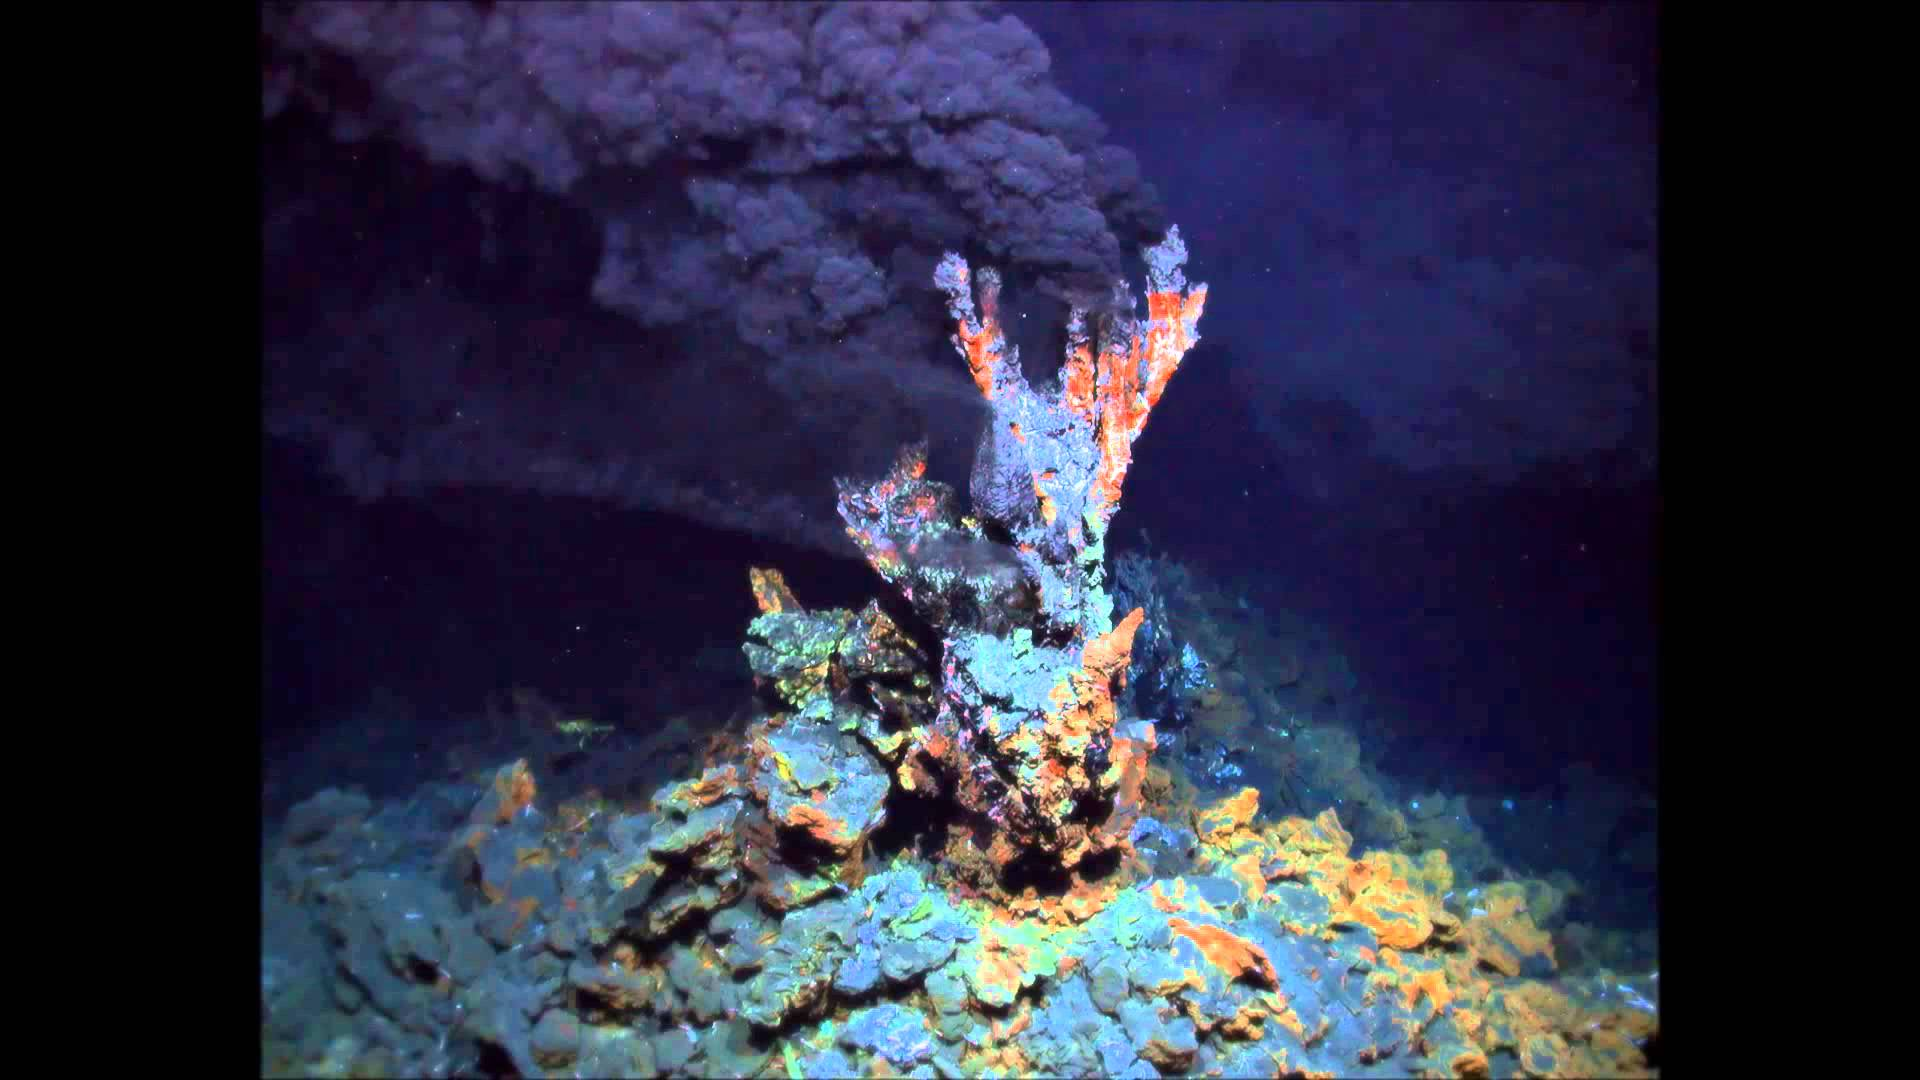
\includegraphics[max width=0.95\textwidth,
        max height=0.48000\textheight]{{Images/hydrothermal}.jpeg}
    \end{center}
    \end{column}
    \end{columns}
}
\end{frame}
\begin{frame}[t]{Round 6 --- Planet Earth --- \mbox{Answer 3}}
\vspace{-0.5em}
\begin{block}{Question}
The ``Great Oxidation Event'' began roughly 2 billion years ago when atmospheric oxygen was produced as a waste product of what biological process?
\end{block}

\visible<2->{
    \begin{columns}[T,totalwidth=\linewidth]
    \begin{column}{0.32\linewidth}
    \begin{block}{Answer}
    Photosynthesis
    \end{block}
    \end{column}
    \begin{column}{0.65\linewidth}
    \begin{center}
    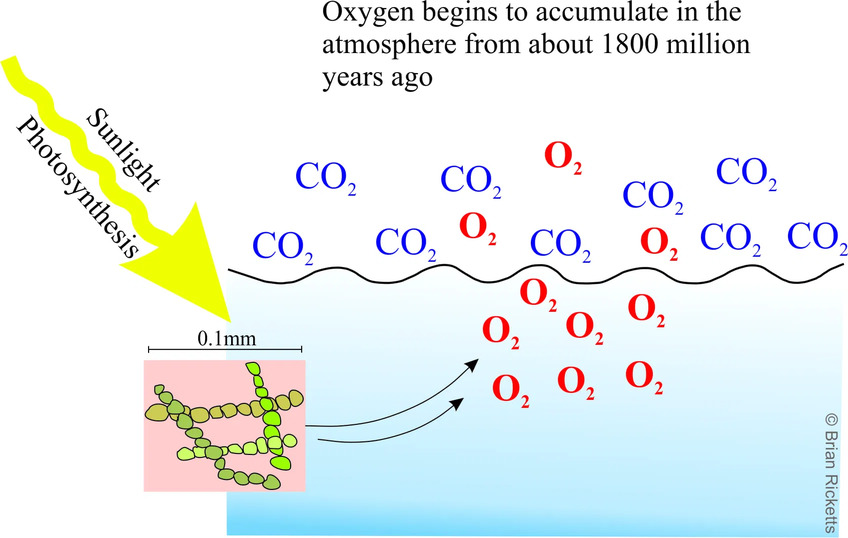
\includegraphics[max width=0.95\textwidth,
        max height=0.48000\textheight]{{Images/oxidation}.jpg}
    \end{center}
    \end{column}
    \end{columns}
}
\end{frame}
\begin{frame}[t]{Round 6 --- Planet Earth --- \mbox{Answer 4}}
\vspace{-0.5em}
\begin{block}{Question}
The radioactive dating method used to determine the age of the oldest rocks on Earth uses the ratio of which two elements to determine the age of a rock?
\end{block}

\visible<2->{
    \begin{columns}[T,totalwidth=\linewidth]
    \begin{column}{0.32\linewidth}
    \begin{block}{Answer}
    Uranium and lead
    \end{block}
    \end{column}
    \begin{column}{0.65\linewidth}
    \begin{center}
    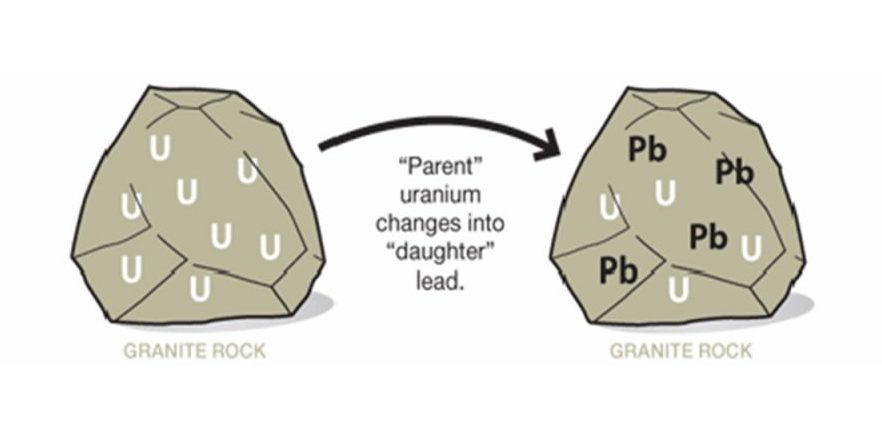
\includegraphics[max width=0.95\textwidth,
        max height=0.43000\textheight]{{Images/uranium}.jpg}
    \end{center}
    \end{column}
    \end{columns}
}
\end{frame}
\begin{frame}[t]{Round 6 --- Planet Earth --- \mbox{Answer 5}}
\vspace{-0.5em}
\begin{block}{Question}
Which layer of the atmosphere is responsible for absorbing much of the Sun's ultraviolet radiation?
\end{block}

\visible<2->{
    \begin{columns}[T,totalwidth=\linewidth]
    \begin{column}{0.32\linewidth}
    \begin{block}{Answer}
    The ozone layer --- we'll also accept stratosphere, as that's the larger layer containing the ozone layer
    \end{block}
    \end{column}
    \begin{column}{0.65\linewidth}
    \begin{center}
    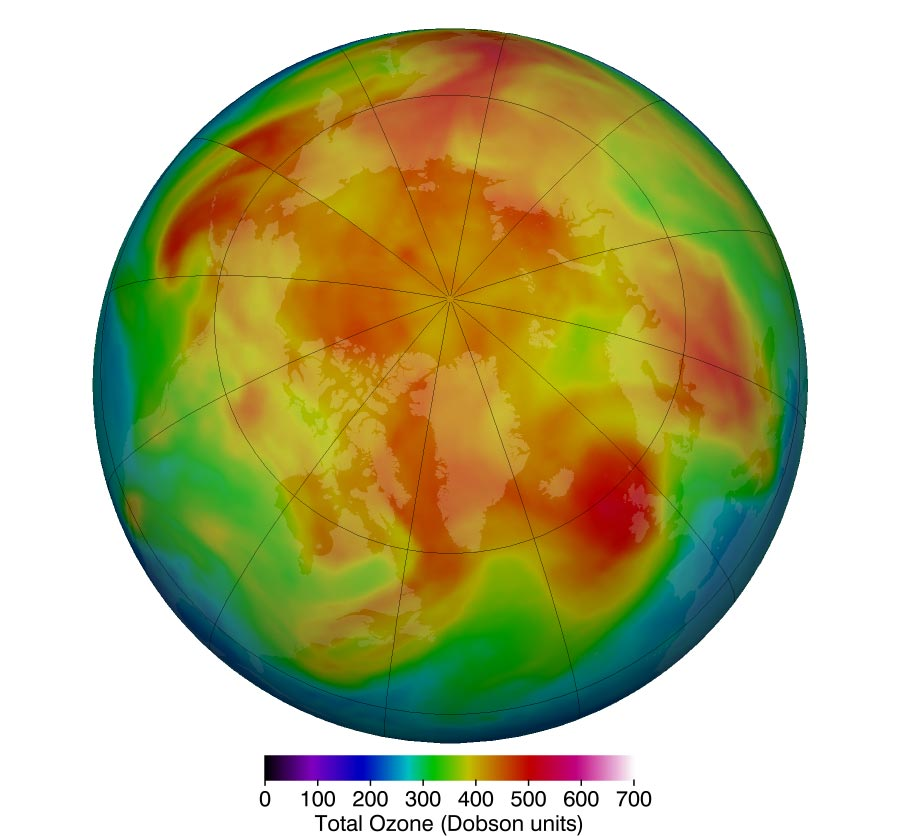
\includegraphics[max width=0.95\textwidth,
        max height=0.53000\textheight]{{Images/ozone}.jpg}
    \end{center}
    \end{column}
    \end{columns}
}
\end{frame}
\begin{frame}[t]{Round 6 --- Planet Earth --- \mbox{Answer 6}}
\vspace{-0.5em}
\begin{block}{Question}
What was the name of the supercontinent that existed from roughly 300 million years ago to 180 million years ago?
\end{block}

\visible<2->{
    \begin{columns}[T,totalwidth=\linewidth]
    \begin{column}{0.32\linewidth}
    \begin{block}{Answer}
    Pangea / Pangaea
    \end{block}
    \end{column}
    \begin{column}{0.65\linewidth}
    \begin{center}
    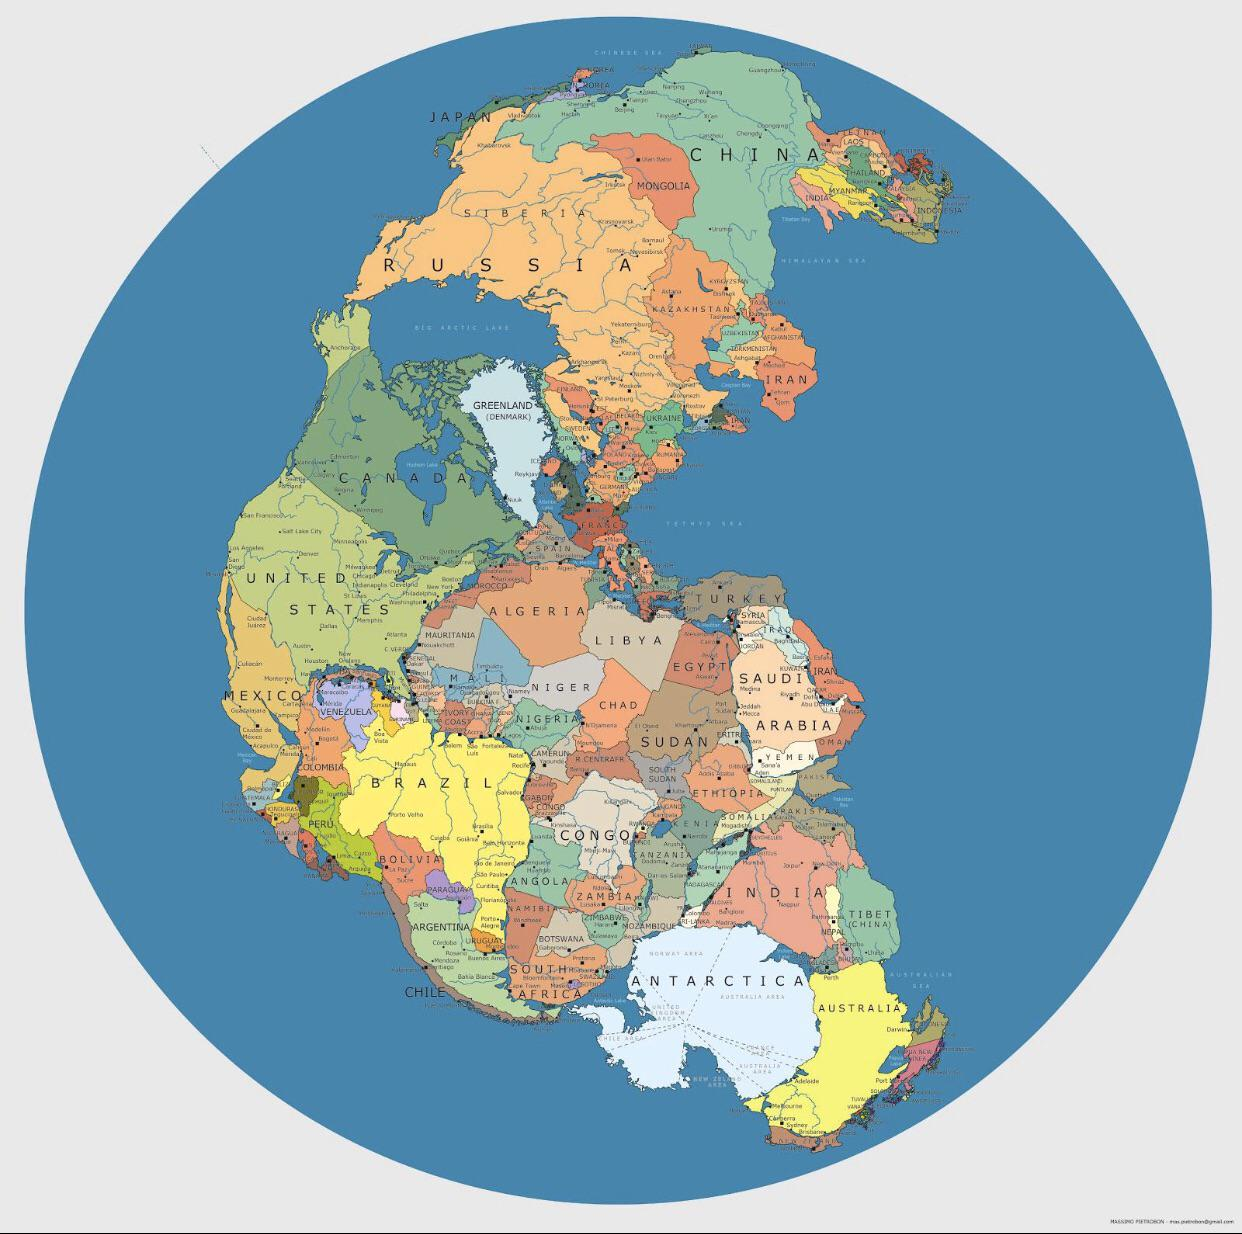
\includegraphics[max width=0.95\textwidth,
        max height=0.48000\textheight]{{Images/pangaea}.jpg}
    \end{center}
    \end{column}
    \end{columns}
}
\end{frame}
\begin{frame}[t]{Round 6 --- Planet Earth --- \mbox{Answer 7}}
\vspace{-0.5em}
\begin{block}{Question}
What was the ``Chicxulub impactor'', which formed the Chicxulub crater in the Yucatan Peninsula?
\end{block}

\visible<2->{
    \begin{columns}[T,totalwidth=\linewidth]
    \begin{column}{0.32\linewidth}
    \begin{block}{Answer}
    The asteroid that wiped out the non-avian dinosaurs (any answer mentioning the extinction of the dinosaurs will be accepted)
    \end{block}
    \end{column}
    \begin{column}{0.65\linewidth}
    \begin{center}
    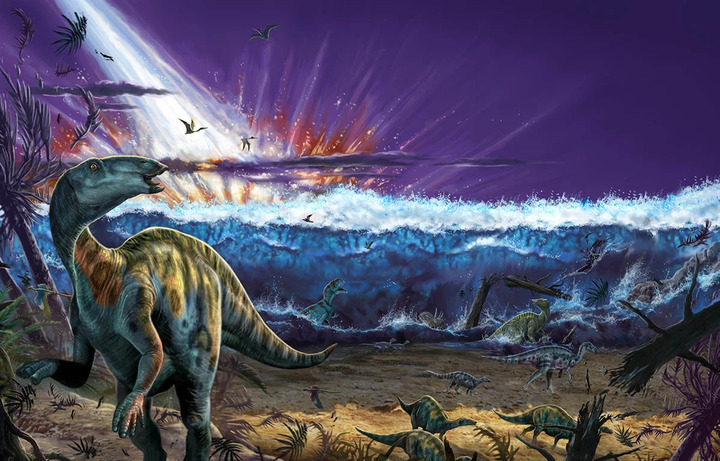
\includegraphics[max width=0.95\textwidth,
        max height=0.53000\textheight]{{Images/chicxulub}.jpg}
    \end{center}
    \end{column}
    \end{columns}
}
\end{frame}
\begin{frame}[t]{Round 6 --- Planet Earth --- \mbox{Answer 8}}
\vspace{-0.5em}
\begin{block}{Question}
The dynamo theory proposes a mechanism by which molten metal in the Earth's center can produce what?
\end{block}

\visible<2->{
    \begin{columns}[T,totalwidth=\linewidth]
    \begin{column}{0.32\linewidth}
    \begin{block}{Answer}
    A magnetic field
    \end{block}
    \end{column}
    \begin{column}{0.65\linewidth}
    \begin{center}
    \includegraphics[max width=0.95\textwidth,
        max height=0.53000\textheight]{{Images/dynamo}.png}
    \end{center}
    \end{column}
    \end{columns}
}
\end{frame}
\begin{frame}[t]{Round 6 --- Planet Earth --- \mbox{Answer 9}}
\vspace{-0.5em}
\begin{block}{Question}
The stream of charged particles released from the Sun out into the solar system, known as solar wind, causes what night-sky natural phenomenon on Earth?
\end{block}

\visible<2->{
    \begin{columns}[T,totalwidth=\linewidth]
    \begin{column}{0.32\linewidth}
    \begin{block}{Answer}
    Auroras / Polar lights / aurora polaris / Northern lights / aurora borealis / Southern lights / aurora australis
    \end{block}
    \end{column}
    \begin{column}{0.65\linewidth}
    \begin{center}
    \includegraphics[max width=0.95\textwidth,
        max height=0.43000\textheight]{{Images/aurora}.jpg}
    \end{center}
    \end{column}
    \end{columns}
}
\end{frame}
\begin{frame}[t]{Round 6 --- Planet Earth --- \mbox{Answer 10}}
\vspace{-0.5em}
\begin{block}{Question}
What is the defining feature of the two lines of latitude known as the Tropic of Cancer and the Tropic of Capricorn?
\end{block}

\visible<2->{
    \begin{columns}[T,totalwidth=\linewidth]
    \begin{column}{0.65\linewidth}
    \begin{block}{Answer}
    They are the farthest latitudes from the equator where the Sun can ever be directly overhead. (On the solstices the Sun will be directly overhead the Tropics.)
    \end{block}
    \end{column}
    \begin{column}{0.3\linewidth}
    \begin{center}
    \includegraphics[max width=0.95\textwidth,
        max height=0.48000\textheight]{{Images/tropics}.jpg}
    \end{center}
    \end{column}
    \end{columns}
}
\end{frame}
\def\thisSectionName{Scandalous Literature}
\section{Round 7}
\subsection*{Q1}
\begin{frame}[t]{Round 7 --- Scandalous Literature --- \mbox{Question 1}}
\vspace{-0.5em}
\begin{block}{Question}
What scandalous novel's plot revolves around an affair between and lady and a gamekeeper?
\end{block}
\end{frame}
\subsection*{Q2}
\begin{frame}[t]{Round 7 --- Scandalous Literature --- \mbox{Question 2}}
\vspace{-0.5em}
\begin{block}{Question}
What scandalous novel's action takes place on June 16, 1904?
\end{block}
\end{frame}
\subsection*{Q3}
\begin{frame}[t]{Round 7 --- Scandalous Literature --- \mbox{Question 3}}
\vspace{-0.5em}
\begin{block}{Question}
What scandalous novel's publication famously led to the issuance of  a fatwah against its author?
\end{block}
\end{frame}
\subsection*{Q4}
\begin{frame}[t]{Round 7 --- Scandalous Literature --- \mbox{Question 4}}
\vspace{-0.5em}
\begin{block}{Question}
The titular character of which scandalous 19\textsuperscript{th} century French novel shares a first name with the titular character of a Jane Austen novel? 
\end{block}
\end{frame}
\subsection*{Q5}
\begin{frame}[t]{Round 7 --- Scandalous Literature --- \mbox{Question 5}}
\vspace{-0.5em}
\begin{block}{Question}
What scandalous 1748 English novel had the alternate title \emph{Memoirs of a Woman of Pleasure}?
\end{block}
\end{frame}
\subsection*{Q6}
\begin{frame}[t]{Round 7 --- Scandalous Literature --- \mbox{Question 6}}
\vspace{-0.5em}
\begin{block}{Question}
What American novel was  first published in Paris in 1934 but, because of its scandalous nature, was not published in the U.S. until 1961? 
\end{block}
\end{frame}
\subsection*{Q7}
\begin{frame}[t]{Round 7 --- Scandalous Literature --- \mbox{Question 7}}
\vspace{-0.5em}
\begin{block}{Question}
What scandalous novel by the Marquis de Sade had the alternate title \emph{The Misfortunes of Virtue}?
\end{block}
\end{frame}
\subsection*{Q8}
\begin{frame}[t]{Round 7 --- Scandalous Literature --- \mbox{Question 8}}
\vspace{-0.5em}
\begin{block}{Question}
Some in Tennessee sought to have this book banned because it stood in part for the proposition that some witches were good. (We need the full name of the book.)
\end{block}
\end{frame}
\subsection*{Q9}
\begin{frame}[t]{Round 7 --- Scandalous Literature --- \mbox{Question 9}}
\vspace{-0.5em}
\begin{block}{Question}
According to the Modern Language Association, what novel was the most banned book in the U.S. during the almost twenty-year period from 1963 to 1982?
\end{block}
\end{frame}
\subsection*{Q10}
\begin{frame}[t]{Round 7 --- Scandalous Literature --- \mbox{Question 10}}
\vspace{-0.5em}
\begin{block}{Question}
What 1960s scandalous Irish trilogy of novels was both popular and critically acclaimed in the United States and England but was banned in the author's home country of Ireland? (We only need the name of the trilogy, not the name of each novel.)
\end{block}
\end{frame}
\subsection{Answers}
\begin{frame}[t]{Round 7 --- Scandalous Literature --- \mbox{Answer 1}}
\vspace{-0.5em}
\begin{block}{Question}
What scandalous novel's plot revolves around an affair between and lady and a gamekeeper?
\end{block}

\visible<2->{
    \begin{columns}[T,totalwidth=\linewidth]
    \begin{column}{0.32\linewidth}
    \begin{block}{Answer}
    \emph{Lady Chatterley's Lover}
    \end{block}
    \end{column}
    \begin{column}{0.65\linewidth}
    \begin{center}
    \includegraphics[max width=0.95\textwidth,
        max height=0.53000\textheight]{{Images/chatterly}.jpeg}
    \end{center}
    \end{column}
    \end{columns}
}
\end{frame}
\begin{frame}[t]{Round 7 --- Scandalous Literature --- \mbox{Answer 2}}
\vspace{-0.5em}
\begin{block}{Question}
What scandalous novel's action takes place on June 16, 1904?
\end{block}

\visible<2->{
    \begin{columns}[T,totalwidth=\linewidth]
    \begin{column}{0.32\linewidth}
    \begin{block}{Answer}
    \emph{Ulysses}
    \end{block}
    \end{column}
    \begin{column}{0.65\linewidth}
    \begin{center}
    \includegraphics[max width=0.95\textwidth,
        max height=0.53000\textheight]{{Images/ulysses}.jpg}
    \end{center}
    \end{column}
    \end{columns}
}
\end{frame}
\begin{frame}[t]{Round 7 --- Scandalous Literature --- \mbox{Answer 3}}
\vspace{-0.5em}
\begin{block}{Question}
What scandalous novel's publication famously led to the issuance of  a fatwah against its author?
\end{block}

\visible<2->{
    \begin{columns}[T,totalwidth=\linewidth]
    \begin{column}{0.32\linewidth}
    \begin{block}{Answer}
    \emph{The Satanic Verses}
    \end{block}
    \end{column}
    \begin{column}{0.65\linewidth}
    \begin{center}
    \includegraphics[max width=0.95\textwidth,
        max height=0.53000\textheight]{{Images/satanic}.jpg}
    \end{center}
    \end{column}
    \end{columns}
}
\end{frame}
\begin{frame}[t]{Round 7 --- Scandalous Literature --- \mbox{Answer 4}}
\vspace{-0.5em}
\begin{block}{Question}
The titular character of which scandalous 19\textsuperscript{th} century French novel shares a first name with the titular character of a Jane Austen novel? 
\end{block}

\visible<2->{
    \begin{columns}[T,totalwidth=\linewidth]
    \begin{column}{0.5\linewidth}
    \begin{block}{Answer}
    \emph{Madame Bovary} (Madame Bovary shares her first name, Emma, with Emma Woodhouse of Austen's novel \emph{Emma})
    \end{block}
    \end{column}
    \begin{column}{0.5\linewidth}
    \begin{center}
    \includegraphics[max width=0.95\textwidth,
        max height=0.43000\textheight]{{Images/bovery}.jpg}
    \end{center}
    \end{column}
    \end{columns}
}
\end{frame}
\begin{frame}[t]{Round 7 --- Scandalous Literature --- \mbox{Answer 5}}
\vspace{-0.5em}
\begin{block}{Question}
What scandalous 1748 English novel had the alternate title \emph{Memoirs of a Woman of Pleasure}?
\end{block}

\visible<2->{
    \begin{columns}[T,totalwidth=\linewidth]
    \begin{column}{0.32\linewidth}
    \begin{block}{Answer}
    \emph{Fanny Hill}
    \end{block}
    \end{column}
    \begin{column}{0.65\linewidth}
    \begin{center}
    \includegraphics[max width=0.95\textwidth,
        max height=0.53000\textheight]{{Images/fannyhill}.jpg}
    \end{center}
    \end{column}
    \end{columns}
}
\end{frame}
\begin{frame}[t]{Round 7 --- Scandalous Literature --- \mbox{Answer 6}}
\vspace{-0.5em}
\begin{block}{Question}
What American novel was  first published in Paris in 1934 but, because of its scandalous nature, was not published in the U.S. until 1961? 
\end{block}

\visible<2->{
    \begin{columns}[T,totalwidth=\linewidth]
    \begin{column}{0.32\linewidth}
    \begin{block}{Answer}
    \emph{Tropic of Cancer}
    \end{block}
    \end{column}
    \begin{column}{0.65\linewidth}
    \begin{center}
    \includegraphics[max width=0.95\textwidth,
        max height=0.48000\textheight]{{Images/tropicofcancer}.jpg}
    \end{center}
    \end{column}
    \end{columns}
}
\end{frame}
\begin{frame}[t]{Round 7 --- Scandalous Literature --- \mbox{Answer 7}}
\vspace{-0.5em}
\begin{block}{Question}
What scandalous novel by the Marquis de Sade had the alternate title \emph{The Misfortunes of Virtue}?
\end{block}

\visible<2->{
    \begin{columns}[T,totalwidth=\linewidth]
    \begin{column}{0.32\linewidth}
    \begin{block}{Answer}
    \emph{Justine}
    \end{block}
    \end{column}
    \begin{column}{0.65\linewidth}
    \begin{center}
    \includegraphics[max width=0.95\textwidth,
        max height=0.48000\textheight]{{Images/justine}.jpg}
    \end{center}
    \end{column}
    \end{columns}
}
\end{frame}
\begin{frame}[t]{Round 7 --- Scandalous Literature --- \mbox{Answer 8}}
\vspace{-0.5em}
\begin{block}{Question}
Some in Tennessee sought to have this book banned because it stood in part for the proposition that some witches were good. (We need the full name of the book.)
\end{block}

\visible<2->{
    \begin{columns}[T,totalwidth=\linewidth]
    \begin{column}{0.32\linewidth}
    \begin{block}{Answer}
    \emph{The Wonderful Wizard of Oz}
    \end{block}
    \end{column}
    \begin{column}{0.65\linewidth}
    \begin{center}
    \includegraphics[max width=0.95\textwidth,
        max height=0.43000\textheight]{{Images/woz}.jpg}
    \end{center}
    \end{column}
    \end{columns}
}
\end{frame}
\begin{frame}[t]{Round 7 --- Scandalous Literature --- \mbox{Answer 9}}
\vspace{-0.5em}
\begin{block}{Question}
According to the Modern Language Association, what novel was the most banned book in the U.S. during the almost twenty-year period from 1963 to 1982?
\end{block}

\visible<2->{
    \begin{columns}[T,totalwidth=\linewidth]
    \begin{column}{0.32\linewidth}
    \begin{block}{Answer}
    \emph{The Catcher in the Rye}
    \end{block}
    \end{column}
    \begin{column}{0.65\linewidth}
    \begin{center}
    \includegraphics[max width=0.95\textwidth,
        max height=0.48000\textheight]{{Images/catcherrye}.jpg}
    \end{center}
    \end{column}
    \end{columns}
}
\end{frame}
\begin{frame}[t]{Round 7 --- Scandalous Literature --- \mbox{Answer 10}}
\vspace{-0.5em}
\begin{block}{Question}
What 1960s scandalous Irish trilogy of novels was both popular and critically acclaimed in the United States and England but was banned in the author's home country of Ireland? (We only need the name of the trilogy, not the name of each novel.)
\end{block}

\visible<2->{
    \begin{columns}[T,totalwidth=\linewidth]
    \begin{column}{0.32\linewidth}
    \begin{block}{Answer}
    \emph{The Country Girls}
    \end{block}
    \end{column}
    \begin{column}{0.65\linewidth}
    \begin{center}
    \includegraphics[max width=0.95\textwidth,
        max height=0.38000\textheight]{{Images/countrygirls}.jpg}
    \end{center}
    \end{column}
    \end{columns}
}
\end{frame}
\def\thisSectionName{The ``Mother of Presidents''}
\section{Round 8}
\subsection*{Q1}
\begin{frame}[t]{Round 8 --- The ``Mother of Presidents'' --- \mbox{Question 1}}
\vspace{-0.5em}
\begin{block}{Question}
Which British monarch was Virginia named for? (We need the monarch's name and numeric suffix.)
\end{block}
\end{frame}
\subsection*{Q2}
\begin{frame}[t]{Round 8 --- The ``Mother of Presidents'' --- \mbox{Question 2}}
\vspace{-0.5em}
\begin{block}{Question}
What infamously-uttered  Latin phrase is also the state motto of Virginia?
\end{block}
\end{frame}
\subsection*{Q3}
\begin{frame}[t]{Round 8 --- The ``Mother of Presidents'' --- \mbox{Question 3}}
\vspace{-0.5em}
\begin{block}{Question}
What is the name of James Monroe's home outside of Charlottesville?
\end{block}
\end{frame}
\subsection*{Q4}
\begin{frame}[t]{Round 8 --- The ``Mother of Presidents'' --- \mbox{Question 4}}
\vspace{-0.5em}
\begin{block}{Question}
Who was the architect of the original part of the University of Virginia?
\end{block}
\end{frame}
\subsection*{Q5}
\begin{frame}[t]{Round 8 --- The ``Mother of Presidents'' --- \mbox{Question 5}}
\vspace{-0.5em}
\begin{block}{Question}
What river runs through Richmond, Virginia?
\end{block}
\end{frame}
\subsection*{Q6}
\begin{frame}[t]{Round 8 --- The ``Mother of Presidents'' --- \mbox{Question 6}}
\vspace{-0.5em}
\begin{block}{Question}
What is the name of the scenic road that runs the length of Shenandoah National Park?
\end{block}
\end{frame}
\subsection*{Q7}
\begin{frame}[t]{Round 8 --- The ``Mother of Presidents'' --- \mbox{Question 7}}
\vspace{-0.5em}
\begin{block}{Question}
Which town located in Virginia was the site of the first British settlement in the New World?
\end{block}
\end{frame}
\subsection*{Q8}
\begin{frame}[t]{Round 8 --- The ``Mother of Presidents'' --- \mbox{Question 8}}
\vspace{-0.5em}
\begin{block}{Question}
What song was retired as Virginia's state song in 1997 because it reflected African-American stereotypes?
\end{block}
\end{frame}
\subsection*{Q9}
\begin{frame}[t]{Round 8 --- The ``Mother of Presidents'' --- \mbox{Question 9}}
\vspace{-0.5em}
\begin{block}{Question}
What is the name of the Virginia governor who was the first U.S. African-American governor of the post-Reconstruction era?
\end{block}
\end{frame}
\subsection*{Q10}
\begin{frame}[t]{Round 8 --- The ``Mother of Presidents'' --- \mbox{Question 10}}
\vspace{-0.5em}
\begin{block}{Question}
What was the name of the  first major battle of the Civil War fought in Virginia?
\end{block}
\end{frame}
\subsection{Answers}
\begin{frame}[t]{Round 8 --- The ``Mother of Presidents'' --- \mbox{Answer 1}}
\vspace{-0.5em}
\begin{block}{Question}
Which British monarch was Virginia named for? (We need the monarch's name and numeric suffix.)
\end{block}

\visible<2->{
    \begin{columns}[T,totalwidth=\linewidth]
    \begin{column}{0.32\linewidth}
    \begin{block}{Answer}
    Elizabeth I (the ``Virgin Queen'')
    \end{block}
    \end{column}
    \begin{column}{0.65\linewidth}
    \begin{center}
    \includegraphics[max width=0.95\textwidth,
        max height=0.53000\textheight]{{Images/qe1}.jpg}
    \end{center}
    \end{column}
    \end{columns}
}
\end{frame}
\begin{frame}[t]{Round 8 --- The ``Mother of Presidents'' --- \mbox{Answer 2}}
\vspace{-0.5em}
\begin{block}{Question}
What infamously-uttered  Latin phrase is also the state motto of Virginia?
\end{block}

\visible<2->{
    \begin{columns}[T,totalwidth=\linewidth]
    \begin{column}{0.65\linewidth}
    \begin{block}{Answer}
    Sic Semper Tyrannis (spelling is not important as long as you got the pronunciation right) --- the phrase was infamously uttered by John Wilkes Booth as he shot Lincoln.
    \end{block}
    \end{column}
    \begin{column}{0.3\linewidth}
    \begin{center}
    \includegraphics[max width=0.95\textwidth,
        max height=0.53000\textheight]{{Images/sicsemper}.jpg}
    \end{center}
    \end{column}
    \end{columns}
}
\end{frame}
\begin{frame}[t]{Round 8 --- The ``Mother of Presidents'' --- \mbox{Answer 3}}
\vspace{-0.5em}
\begin{block}{Question}
What is the name of James Monroe's home outside of Charlottesville?
\end{block}

\visible<2->{
    \begin{columns}[T,totalwidth=\linewidth]
    \begin{column}{0.32\linewidth}
    \begin{block}{Answer}
    Highland / Ash Lawn / Ash Lawn--Highland 
    \end{block}
    \end{column}
    \begin{column}{0.65\linewidth}
    \begin{center}
    \includegraphics[max width=0.95\textwidth,
        max height=0.53000\textheight]{{Images/highland}.jpg}
    \end{center}
    \end{column}
    \end{columns}
}
\end{frame}
\begin{frame}[t]{Round 8 --- The ``Mother of Presidents'' --- \mbox{Answer 4}}
\vspace{-0.5em}
\begin{block}{Question}
Who was the architect of the original part of the University of Virginia?
\end{block}

\visible<2->{
    \begin{columns}[T,totalwidth=\linewidth]
    \begin{column}{0.32\linewidth}
    \begin{block}{Answer}
    Thomas Jefferson
    \end{block}
    \end{column}
    \begin{column}{0.65\linewidth}
    \begin{center}
    \includegraphics[max width=0.95\textwidth,
        max height=0.53000\textheight]{{Images/tj}.jpg}
    \end{center}
    \end{column}
    \end{columns}
}
\end{frame}
\begin{frame}[t]{Round 8 --- The ``Mother of Presidents'' --- \mbox{Answer 5}}
\vspace{-0.5em}
\begin{block}{Question}
What river runs through Richmond, Virginia?
\end{block}

\visible<2->{
    \begin{columns}[T,totalwidth=\linewidth]
    \begin{column}{0.32\linewidth}
    \begin{block}{Answer}
    The James River
    \end{block}
    \end{column}
    \begin{column}{0.65\linewidth}
    \begin{center}
    \includegraphics[max width=0.95\textwidth,
        max height=0.58000\textheight]{{Images/jamesriver}.jpg}
    \end{center}
    \end{column}
    \end{columns}
}
\end{frame}
\begin{frame}[t]{Round 8 --- The ``Mother of Presidents'' --- \mbox{Answer 6}}
\vspace{-0.5em}
\begin{block}{Question}
What is the name of the scenic road that runs the length of Shenandoah National Park?
\end{block}

\visible<2->{
    \begin{columns}[T,totalwidth=\linewidth]
    \begin{column}{0.32\linewidth}
    \begin{block}{Answer}
    The Skyline Drive
    \end{block}
    \end{column}
    \begin{column}{0.65\linewidth}
    \begin{center}
    \includegraphics[max width=0.95\textwidth,
        max height=0.53000\textheight]{{Images/skyline}.jpg}
    \end{center}
    \end{column}
    \end{columns}
}
\end{frame}
\begin{frame}[t]{Round 8 --- The ``Mother of Presidents'' --- \mbox{Answer 7}}
\vspace{-0.5em}
\begin{block}{Question}
Which town located in Virginia was the site of the first British settlement in the New World?
\end{block}

\visible<2->{
    \begin{columns}[T,totalwidth=\linewidth]
    \begin{column}{0.32\linewidth}
    \begin{block}{Answer}
    Jamestown
    \end{block}
    \end{column}
    \begin{column}{0.65\linewidth}
    \begin{center}
    \includegraphics[max width=0.95\textwidth,
        max height=0.53000\textheight]{{Images/jamestown}.jpg}
    \end{center}
    \end{column}
    \end{columns}
}
\end{frame}
\begin{frame}[t]{Round 8 --- The ``Mother of Presidents'' --- \mbox{Answer 8}}
\vspace{-0.5em}
\begin{block}{Question}
What song was retired as Virginia's state song in 1997 because it reflected African-American stereotypes?
\end{block}

\visible<2->{
    \begin{columns}[T,totalwidth=\linewidth]
    \begin{column}{0.32\linewidth}
    \begin{block}{Answer}
    Carry Me Back to Old Virginny
    \end{block}
    \end{column}
    \begin{column}{0.65\linewidth}
    \begin{center}
    \includegraphics[max width=0.95\textwidth,
        max height=0.48000\textheight]{{Images/virginny}.jpg}
    \end{center}
    \end{column}
    \end{columns}
}
\end{frame}
\begin{frame}[t]{Round 8 --- The ``Mother of Presidents'' --- \mbox{Answer 9}}
\vspace{-0.5em}
\begin{block}{Question}
What is the name of the Virginia governor who was the first U.S. African-American governor of the post-Reconstruction era?
\end{block}

\visible<2->{
    \begin{columns}[T,totalwidth=\linewidth]
    \begin{column}{0.32\linewidth}
    \begin{block}{Answer}
    Douglas Wilder
    \end{block}
    \end{column}
    \begin{column}{0.65\linewidth}
    \begin{center}
    \includegraphics[max width=0.95\textwidth,
        max height=0.48000\textheight]{{Images/wilder}.jpg}
    \end{center}
    \end{column}
    \end{columns}
}
\end{frame}
\begin{frame}[t]{Round 8 --- The ``Mother of Presidents'' --- \mbox{Answer 10}}
\vspace{-0.5em}
\begin{block}{Question}
What was the name of the  first major battle of the Civil War fought in Virginia?
\end{block}

\visible<2->{
    \begin{columns}[T,totalwidth=\linewidth]
    \begin{column}{0.32\linewidth}
    \begin{block}{Answer}
    The First Battle of Bull Run / The Battle of First Manassas
    \end{block}
    \end{column}
    \begin{column}{0.65\linewidth}
    \begin{center}
    \includegraphics[max width=0.95\textwidth,
        max height=0.53000\textheight]{{Images/bullrun}.jpg}
    \end{center}
    \end{column}
    \end{columns}
}
\end{frame}
\def\thisSectionName{Who Directed It?}
\section{Round 9}
\subsection*{Q1}
\begin{frame}[t]{Round 9 --- Who Directed It? --- \mbox{Question 1}}
\vspace{-0.5em}
\begin{block}{Question}
\emph{Bonnie and Clyde} (1967)
\end{block}
\end{frame}
\subsection*{Q2}
\begin{frame}[t]{Round 9 --- Who Directed It? --- \mbox{Question 2}}
\vspace{-0.5em}
\begin{block}{Question}
\emph{American Graffiti} (1973)
\end{block}
\end{frame}
\subsection*{Q3}
\begin{frame}[t]{Round 9 --- Who Directed It? --- \mbox{Question 3}}
\vspace{-0.5em}
\begin{block}{Question}
\emph{Casablanca} (1942)
\end{block}
\end{frame}
\subsection*{Q4}
\begin{frame}[t]{Round 9 --- Who Directed It? --- \mbox{Question 4}}
\vspace{-0.5em}
\begin{block}{Question}
\emph{Jurassic Park} (1993)
\end{block}
\end{frame}
\subsection*{Q5}
\begin{frame}[t]{Round 9 --- Who Directed It? --- \mbox{Question 5}}
\vspace{-0.5em}
\begin{block}{Question}
\emph{F for Fake} (1973)
\end{block}
\end{frame}
\subsection*{Q6}
\begin{frame}[t]{Round 9 --- Who Directed It? --- \mbox{Question 6}}
\vspace{-0.5em}
\begin{block}{Question}
\emph{Dr.\ No} (1962)
\end{block}
\end{frame}
\subsection*{Q7}
\begin{frame}[t]{Round 9 --- Who Directed It? --- \mbox{Question 7}}
\vspace{-0.5em}
\begin{block}{Question}
\emph{It Happened One Night} (1934)
\end{block}
\end{frame}
\subsection*{Q8}
\begin{frame}[t]{Round 9 --- Who Directed It? --- \mbox{Question 8}}
\vspace{-0.5em}
\begin{block}{Question}
\emph{Help!} (1965)
\end{block}
\end{frame}
\subsection*{Q9}
\begin{frame}[t]{Round 9 --- Who Directed It? --- \mbox{Question 9}}
\vspace{-0.5em}
\begin{block}{Question}
\emph{Monsieur Verdoux} (1947)
\end{block}
\end{frame}
\subsection*{Q10}
\begin{frame}[t]{Round 9 --- Who Directed It? --- \mbox{Question 10}}
\vspace{-0.5em}
\begin{block}{Question}
\emph{Black Panther} (2018)
\end{block}
\end{frame}
\subsection{Answers}
\begin{frame}[t]{Round 9 --- Who Directed It? --- \mbox{Answer 1}}
\vspace{-0.5em}
\begin{block}{Question}
\emph{Bonnie and Clyde} (1967)
\end{block}

\visible<2->{
    \begin{columns}[T,totalwidth=\linewidth]
    \begin{column}{0.32\linewidth}
    \begin{block}{Answer}
    Arthur Penn
    \end{block}
    \end{column}
    \begin{column}{0.65\linewidth}
    \begin{center}
    \includegraphics[max width=0.95\textwidth,
        max height=0.58000\textheight]{{Images/bonnieclyde}.jpg}
    \end{center}
    \end{column}
    \end{columns}
}
\end{frame}
\begin{frame}[t]{Round 9 --- Who Directed It? --- \mbox{Answer 2}}
\vspace{-0.5em}
\begin{block}{Question}
\emph{American Graffiti} (1973)
\end{block}

\visible<2->{
    \begin{columns}[T,totalwidth=\linewidth]
    \begin{column}{0.32\linewidth}
    \begin{block}{Answer}
    George Lucas
    \end{block}
    \end{column}
    \begin{column}{0.65\linewidth}
    \begin{center}
    \includegraphics[max width=0.95\textwidth,
        max height=0.58000\textheight]{{Images/georgelucas}.jpg}
    \end{center}
    \end{column}
    \end{columns}
}
\end{frame}
\begin{frame}[t]{Round 9 --- Who Directed It? --- \mbox{Answer 3}}
\vspace{-0.5em}
\begin{block}{Question}
\emph{Casablanca} (1942)
\end{block}

\visible<2->{
    \begin{columns}[T,totalwidth=\linewidth]
    \begin{column}{0.32\linewidth}
    \begin{block}{Answer}
    Michael Curtiz
    \end{block}
    \end{column}
    \begin{column}{0.65\linewidth}
    \begin{center}
    \includegraphics[max width=0.95\textwidth,
        max height=0.58000\textheight]{{Images/casablanca}.jpg}
    \end{center}
    \end{column}
    \end{columns}
}
\end{frame}
\begin{frame}[t]{Round 9 --- Who Directed It? --- \mbox{Answer 4}}
\vspace{-0.5em}
\begin{block}{Question}
\emph{Jurassic Park} (1993)
\end{block}

\visible<2->{
    \begin{columns}[T,totalwidth=\linewidth]
    \begin{column}{0.32\linewidth}
    \begin{block}{Answer}
    Steven Spielberg
    \end{block}
    \end{column}
    \begin{column}{0.65\linewidth}
    \begin{center}
    \includegraphics[max width=0.95\textwidth,
        max height=0.58000\textheight]{{Images/jurassic}.jpg}
    \end{center}
    \end{column}
    \end{columns}
}
\end{frame}
\begin{frame}[t]{Round 9 --- Who Directed It? --- \mbox{Answer 5}}
\vspace{-0.5em}
\begin{block}{Question}
\emph{F for Fake} (1973)
\end{block}

\visible<2->{
    \begin{columns}[T,totalwidth=\linewidth]
    \begin{column}{0.32\linewidth}
    \begin{block}{Answer}
    Orson Welles
    \end{block}
    \end{column}
    \begin{column}{0.65\linewidth}
    \begin{center}
    \includegraphics[max width=0.95\textwidth,
        max height=0.58000\textheight]{{Images/fforfake}.jpg}
    \end{center}
    \end{column}
    \end{columns}
}
\end{frame}
\begin{frame}[t]{Round 9 --- Who Directed It? --- \mbox{Answer 6}}
\vspace{-0.5em}
\begin{block}{Question}
\emph{Dr.\ No} (1962)
\end{block}

\visible<2->{
    \begin{columns}[T,totalwidth=\linewidth]
    \begin{column}{0.32\linewidth}
    \begin{block}{Answer}
    Terence Young
    \end{block}
    \end{column}
    \begin{column}{0.65\linewidth}
    \begin{center}
    \includegraphics[max width=0.95\textwidth,
        max height=0.58000\textheight]{{Images/drno}.jpg}
    \end{center}
    \end{column}
    \end{columns}
}
\end{frame}
\begin{frame}[t]{Round 9 --- Who Directed It? --- \mbox{Answer 7}}
\vspace{-0.5em}
\begin{block}{Question}
\emph{It Happened One Night} (1934)
\end{block}

\visible<2->{
    \begin{columns}[T,totalwidth=\linewidth]
    \begin{column}{0.32\linewidth}
    \begin{block}{Answer}
    Frank Capra
    \end{block}
    \end{column}
    \begin{column}{0.65\linewidth}
    \begin{center}
    \includegraphics[max width=0.95\textwidth,
        max height=0.58000\textheight]{{Images/onenight}.jpg}
    \end{center}
    \end{column}
    \end{columns}
}
\end{frame}
\begin{frame}[t]{Round 9 --- Who Directed It? --- \mbox{Answer 8}}
\vspace{-0.5em}
\begin{block}{Question}
\emph{Help!} (1965)
\end{block}

\visible<2->{
    \begin{columns}[T,totalwidth=\linewidth]
    \begin{column}{0.32\linewidth}
    \begin{block}{Answer}
    Richard Lester
    \end{block}
    \end{column}
    \begin{column}{0.65\linewidth}
    \begin{center}
    \includegraphics[max width=0.95\textwidth,
        max height=0.58000\textheight]{{Images/help}.jpg}
    \end{center}
    \end{column}
    \end{columns}
}
\end{frame}
\begin{frame}[t]{Round 9 --- Who Directed It? --- \mbox{Answer 9}}
\vspace{-0.5em}
\begin{block}{Question}
\emph{Monsieur Verdoux} (1947)
\end{block}

\visible<2->{
    \begin{columns}[T,totalwidth=\linewidth]
    \begin{column}{0.32\linewidth}
    \begin{block}{Answer}
    Charlie Chaplin
    \end{block}
    \end{column}
    \begin{column}{0.65\linewidth}
    \begin{center}
    \includegraphics[max width=0.95\textwidth,
        max height=0.58000\textheight]{{Images/verdoux}.jpg}
    \end{center}
    \end{column}
    \end{columns}
}
\end{frame}
\begin{frame}[t]{Round 9 --- Who Directed It? --- \mbox{Answer 10}}
\vspace{-0.5em}
\begin{block}{Question}
\emph{Black Panther} (2018)
\end{block}

\visible<2->{
    \begin{columns}[T,totalwidth=\linewidth]
    \begin{column}{0.32\linewidth}
    \begin{block}{Answer}
    Ryan Coogler
    \end{block}
    \end{column}
    \begin{column}{0.65\linewidth}
    \begin{center}
    \includegraphics[max width=0.95\textwidth,
        max height=0.58000\textheight]{{Images/coogler}.jpg}
    \end{center}
    \end{column}
    \end{columns}
}
\end{frame}
\def\thisSectionName{``Royals''}
\section{Round 10}
\subsection*{Q1}
\begin{frame}[t]{Round 10 --- ``Royals'' --- \mbox{Question 1}}
\vspace{-0.5em}
\begin{block}{Question}
Which Newark-born rapper and actress's first album was titled \emph{All Hail the Queen}?
\end{block}
\end{frame}
\subsection*{Q2}
\begin{frame}[t]{Round 10 --- ``Royals'' --- \mbox{Question 2}}
\vspace{-0.5em}
\begin{block}{Question}
Which musical artist's first hit was the song \emph{Sweet Lorraine}?
\end{block}
\end{frame}
\subsection*{Q3}
\begin{frame}[t]{Round 10 --- ``Royals'' --- \mbox{Question 3}}
\vspace{-0.5em}
\begin{block}{Question}
Which brand of tobacco formed the basis of a telephone prank whose punchline was ``Well, you'd better let him out!''?
\end{block}
\end{frame}
\subsection*{Q4}
\begin{frame}[t]{Round 10 --- ``Royals'' --- \mbox{Question 4}}
\vspace{-0.5em}
\begin{block}{Question}
Which shock jock has proclaimed himself ``King of All Media'' and, indeed, has trademarked that phrase?
\end{block}
\end{frame}
\subsection*{Q5}
\begin{frame}[t]{Round 10 --- ``Royals'' --- \mbox{Question 5}}
\vspace{-0.5em}
\begin{block}{Question}
Which French-American rock band is best-known for their hit song ``Dancing in the Moonlight''?
\end{block}
\end{frame}
\subsection*{Q6}
\begin{frame}[t]{Round 10 --- ``Royals'' --- \mbox{Question 6}}
\vspace{-0.5em}
\begin{block}{Question}
What noble title did singer Gene Chandler confer upon himself in a 1960s doo-wop hit song?
\end{block}
\end{frame}
\subsection*{Q7}
\begin{frame}[t]{Round 10 --- ``Royals'' --- \mbox{Question 7}}
\vspace{-0.5em}
\begin{block}{Question}
Rogers and Nelson were the middle and last names of which artist who was known by his first name?
\end{block}
\end{frame}
\subsection*{Q8}
\begin{frame}[t]{Round 10 --- ``Royals'' --- \mbox{Question 8}}
\vspace{-0.5em}
\begin{block}{Question}
A resident of Yonkers, NY, has filed a suit against which baked goods company because their rolls are not actually made in Hawaii?
\end{block}
\end{frame}
\subsection*{Q9}
\begin{frame}[t]{Round 10 --- ``Royals'' --- \mbox{Question 9}}
\vspace{-0.5em}
\begin{block}{Question}
What was the title of Queen's first album?
\end{block}
\end{frame}
\subsection*{Q10}
\begin{frame}[t]{Round 10 --- ``Royals'' --- \mbox{Question 10}}
\vspace{-0.5em}
\begin{block}{Question}
Which singer-songwriter entered the music scene in 2018 with her hit single ``1950'' and released her debut studio album, \emph{Cheap Queen}, in 2019?
\end{block}
\end{frame}
\subsection{Answers}
\begin{frame}[t]{Round 10 --- ``Royals'' --- \mbox{Answer 1}}
\vspace{-0.5em}
\begin{block}{Question}
Which Newark-born rapper and actress's first album was titled \emph{All Hail the Queen}?
\end{block}

\visible<2->{
    \begin{columns}[T,totalwidth=\linewidth]
    \begin{column}{0.32\linewidth}
    \begin{block}{Answer}
    Queen Latifah
    \end{block}
    \end{column}
    \begin{column}{0.65\linewidth}
    \begin{center}
    \includegraphics[max width=0.95\textwidth,
        max height=0.53000\textheight]{{Images/latifah}.jpg}
    \end{center}
    \end{column}
    \end{columns}
}
\end{frame}
\begin{frame}[t]{Round 10 --- ``Royals'' --- \mbox{Answer 2}}
\vspace{-0.5em}
\begin{block}{Question}
Which musical artist's first hit was the song \emph{Sweet Lorraine}?
\end{block}

\visible<2->{
    \begin{columns}[T,totalwidth=\linewidth]
    \begin{column}{0.32\linewidth}
    \begin{block}{Answer}
    Nat King Cole
    \end{block}
    \end{column}
    \begin{column}{0.65\linewidth}
    \begin{center}
    \includegraphics[max width=0.95\textwidth,
        max height=0.53000\textheight]{{Images/cole}.jpg}
    \end{center}
    \end{column}
    \end{columns}
}
\end{frame}
\begin{frame}[t]{Round 10 --- ``Royals'' --- \mbox{Answer 3}}
\vspace{-0.5em}
\begin{block}{Question}
Which brand of tobacco formed the basis of a telephone prank whose punchline was ``Well, you'd better let him out!''?
\end{block}

\visible<2->{
    \begin{columns}[T,totalwidth=\linewidth]
    \begin{column}{0.32\linewidth}
    \begin{block}{Answer}
    Prince Albert / Prince Albert in a Can
    \end{block}
    \end{column}
    \begin{column}{0.65\linewidth}
    \begin{center}
    \includegraphics[max width=0.95\textwidth,
        max height=0.48000\textheight]{{Images/princealbert}.jpg}
    \end{center}
    \end{column}
    \end{columns}
}
\end{frame}
\begin{frame}[t]{Round 10 --- ``Royals'' --- \mbox{Answer 4}}
\vspace{-0.5em}
\begin{block}{Question}
Which shock jock has proclaimed himself ``King of All Media'' and, indeed, has trademarked that phrase?
\end{block}

\visible<2->{
    \begin{columns}[T,totalwidth=\linewidth]
    \begin{column}{0.32\linewidth}
    \begin{block}{Answer}
    Howard Stern
    \end{block}
    \end{column}
    \begin{column}{0.65\linewidth}
    \begin{center}
    \includegraphics[max width=0.95\textwidth,
        max height=0.48000\textheight]{{Images/stern}.jpg}
    \end{center}
    \end{column}
    \end{columns}
}
\end{frame}
\begin{frame}[t]{Round 10 --- ``Royals'' --- \mbox{Answer 5}}
\vspace{-0.5em}
\begin{block}{Question}
Which French-American rock band is best-known for their hit song ``Dancing in the Moonlight''?
\end{block}

\visible<2->{
    \begin{columns}[T,totalwidth=\linewidth]
    \begin{column}{0.32\linewidth}
    \begin{block}{Answer}
    King Harvest
    \end{block}
    \end{column}
    \begin{column}{0.65\linewidth}
    \begin{center}
    \includegraphics[max width=0.95\textwidth,
        max height=0.53000\textheight]{{Images/kingharvest}.jpg}
    \end{center}
    \end{column}
    \end{columns}
}
\end{frame}
\begin{frame}[t]{Round 10 --- ``Royals'' --- \mbox{Answer 6}}
\vspace{-0.5em}
\begin{block}{Question}
What noble title did singer Gene Chandler confer upon himself in a 1960s doo-wop hit song?
\end{block}

\visible<2->{
    \begin{columns}[T,totalwidth=\linewidth]
    \begin{column}{0.32\linewidth}
    \begin{block}{Answer}
    Duke of Earl
    \end{block}
    \end{column}
    \begin{column}{0.65\linewidth}
    \begin{center}
    \includegraphics[max width=0.95\textwidth,
        max height=0.53000\textheight]{{Images/dukeofearl}.jpg}
    \end{center}
    \end{column}
    \end{columns}
}
\end{frame}
\begin{frame}[t]{Round 10 --- ``Royals'' --- \mbox{Answer 7}}
\vspace{-0.5em}
\begin{block}{Question}
Rogers and Nelson were the middle and last names of which artist who was known by his first name?
\end{block}

\visible<2->{
    \begin{columns}[T,totalwidth=\linewidth]
    \begin{column}{0.32\linewidth}
    \begin{block}{Answer}
    Prince
    \end{block}
    \end{column}
    \begin{column}{0.65\linewidth}
    \begin{center}
    \includegraphics[max width=0.95\textwidth,
        max height=0.53000\textheight]{{Images/prince}.jpeg}
    \end{center}
    \end{column}
    \end{columns}
}
\end{frame}
\begin{frame}[t]{Round 10 --- ``Royals'' --- \mbox{Answer 8}}
\vspace{-0.5em}
\begin{block}{Question}
A resident of Yonkers, NY, has filed a suit against which baked goods company because their rolls are not actually made in Hawaii?
\end{block}

\visible<2->{
    \begin{columns}[T,totalwidth=\linewidth]
    \begin{column}{0.32\linewidth}
    \begin{block}{Answer}
    King's Hawaiian
    \end{block}
    \end{column}
    \begin{column}{0.65\linewidth}
    \begin{center}
    \includegraphics[max width=0.95\textwidth,
        max height=0.48000\textheight]{{Images/kingshawaiian}.jpeg}
    \end{center}
    \end{column}
    \end{columns}
}
\end{frame}
\begin{frame}[t]{Round 10 --- ``Royals'' --- \mbox{Answer 9}}
\vspace{-0.5em}
\begin{block}{Question}
What was the title of Queen's first album?
\end{block}

\visible<2->{
    \begin{columns}[T,totalwidth=\linewidth]
    \begin{column}{0.32\linewidth}
    \begin{block}{Answer}
    \emph{Queen}
    \end{block}
    \end{column}
    \begin{column}{0.65\linewidth}
    \begin{center}
    \includegraphics[max width=0.95\textwidth,
        max height=0.58000\textheight]{{Images/queen}.jpg}
    \end{center}
    \end{column}
    \end{columns}
}
\end{frame}
\begin{frame}[t]{Round 10 --- ``Royals'' --- \mbox{Answer 10}}
\vspace{-0.5em}
\begin{block}{Question}
Which singer-songwriter entered the music scene in 2018 with her hit single ``1950'' and released her debut studio album, \emph{Cheap Queen}, in 2019?
\end{block}

\visible<2->{
    \begin{columns}[T,totalwidth=\linewidth]
    \begin{column}{0.32\linewidth}
    \begin{block}{Answer}
    King Princess
    \end{block}
    \end{column}
    \begin{column}{0.65\linewidth}
    \begin{center}
    \includegraphics[max width=0.95\textwidth,
        max height=0.48000\textheight]{{Images/kingprincess}.jpg}
    \end{center}
    \end{column}
    \end{columns}
}
\end{frame}
\def\thisSectionName{Bonus}
\section{Bonus Round}
\subsection*{Q1}
\begin{frame}[t]{Bonus Round --- .org}
\vspace{-0.5em}
\begin{block}{Question}
Which American organization's motto is ``We are their voice''?
\end{block}
\end{frame}
\subsection*{Q2}
\begin{frame}[t]{Bonus Round --- Answer Like It's 1999}
\vspace{-0.5em}
\begin{block}{Question}
Which country won the 1999 Women's FIFA World Cup?
\end{block}
\end{frame}
\subsection*{Q3}
\begin{frame}[t]{Bonus Round --- Count On It}
\vspace{-0.5em}
\begin{block}{Question}
To within one, how many presidents, current or former, had previously served as vice president?
\end{block}
\end{frame}
\subsection*{Q4}
\begin{frame}[t]{Bonus Round --- Ham's Solo}
\vspace{-0.5em}
\begin{block}{Question}
[Fill in all three blanks]\\
The fair Ophelia! Nymph, in thy orisons\\
Be all \textunderscore{}\textunderscore{}\textunderscore{}\textunderscore{}\textunderscore{} \textunderscore{}\textunderscore{}\textunderscore{}\textunderscore{}\textunderscore{} \textunderscore{}\textunderscore{}\textunderscore{}\textunderscore{}\textunderscore{}.
\end{block}
\end{frame}
\subsection*{Q5}
\begin{frame}[t]{Bonus Round --- Philosophy and Philosophers}
\vspace{-0.5em}
\begin{block}{Question}
Which lawyer-cum-social philosopher wrote a satirical book about a fictional island whose name literally means ``nowhere'' in Greek? (The name of the island has since come to mean something else in English.)
\end{block}
\end{frame}
\subsection*{Q6}
\begin{frame}[t]{Bonus Round --- Planet Earth}
\vspace{-0.5em}
\begin{block}{Question}
A shipment of toys that fell off a ship in 1992 and began to wash up on beaches around the world significantly helped oceanographers in mapping out the oceans' currents. What kind of toys fell overboard?
\end{block}
\end{frame}
\subsection*{Q7}
\begin{frame}[t]{Bonus Round --- Scandalous Literature}
\vspace{-0.5em}
\begin{block}{Question}
The reaction to what 1975 young adult novel caused its author to say, ``Parents are getting cuckoo''?
\end{block}
\end{frame}
\subsection*{Q8}
\begin{frame}[t]{Bonus Round --- The ``Mother of Presidents''}
\vspace{-0.5em}
\begin{block}{Question}
How many presidents were born in Virginia (either the colony or the commonwealth)?
\end{block}
\end{frame}
\subsection*{Q9}
\begin{frame}[t]{Bonus Round --- Who Directed It?}
\vspace{-0.5em}
\begin{block}{Question}
\emph{A Night at the Opera} (1935)
\end{block}
\end{frame}
\subsection*{Q10}
\begin{frame}[t]{Bonus Round --- ``Royals''}
\vspace{-0.5em}
\begin{block}{Question}
Who were the two famous piano-playing big band leaders of the 20\textsuperscript{th} century who were known by titles of nobility? (We need both names.)
\end{block}
\end{frame}
\subsection{Answers}
\begin{frame}[t]{Bonus Round --- .org}
\vspace{-0.5em}
\begin{block}{Question}
Which American organization's motto is ``We are their voice''?
\end{block}

\visible<2->{
    \begin{columns}[T,totalwidth=\linewidth]
    \begin{column}{0.32\linewidth}
    \begin{block}{Answer}
    The ASPCA (American Society for the Prevention of Cruelty to Animals)
    \end{block}
    \end{column}
    \begin{column}{0.65\linewidth}
    \begin{center}
    \includegraphics[max width=0.95\textwidth,
        max height=0.53000\textheight]{{Images/aspca}.png}
    \end{center}
    \end{column}
    \end{columns}
}
\end{frame}
\begin{frame}[t]{Bonus Round --- Answer Like It's 1999}
\vspace{-0.5em}
\begin{block}{Question}
Which country won the 1999 Women's FIFA World Cup?
\end{block}

\visible<2->{
    \begin{columns}[T,totalwidth=\linewidth]
    \begin{column}{0.32\linewidth}
    \begin{block}{Answer}
    The U.S.
    \end{block}
    \end{column}
    \begin{column}{0.65\linewidth}
    \begin{center}
    \includegraphics[max width=0.95\textwidth,
        max height=0.58000\textheight]{{Images/hamm}.jpg}
    \end{center}
    \end{column}
    \end{columns}
}
\end{frame}
\begin{frame}[t]{Bonus Round --- Count On It}
\vspace{-0.5em}
\begin{block}{Question}
To within one, how many presidents, current or former, had previously served as vice president?
\end{block}

\visible<2->{
    \begin{columns}[T,totalwidth=\linewidth]
    \begin{column}{0.32\linewidth}
    \begin{block}{Answer}
    Fifteen (14--16 will be accepted) (JA, TJ, MvB, JT, MF, AJ, CAA, TR, CC, HST, RN, LBJ, GF, GHWB, JB)
    \end{block}
    \end{column}
    \begin{column}{0.65\linewidth}
    \begin{center}
    \includegraphics[max width=0.95\textwidth,
        max height=0.53000\textheight]{{Images/vps}.jpg}
    \end{center}
    \end{column}
    \end{columns}
}
\end{frame}
\begin{frame}[t]{Bonus Round --- Ham's Solo}
\vspace{-0.5em}
\begin{block}{Question}
[Fill in all three blanks]\\
The fair Ophelia! Nymph, in thy orisons\\
Be all \textunderscore{}\textunderscore{}\textunderscore{}\textunderscore{}\textunderscore{} \textunderscore{}\textunderscore{}\textunderscore{}\textunderscore{}\textunderscore{} \textunderscore{}\textunderscore{}\textunderscore{}\textunderscore{}\textunderscore{}.
\end{block}
\visible<2->{
    \begin{block}{Answer}
    My sins remember'd (``remembered'' without the apostrophe is fine)
    \end{block}
}
\end{frame}
\begin{frame}[t]{Bonus Round --- Philosophy and Philosophers}
\vspace{-0.5em}
\begin{block}{Question}
Which lawyer-cum-social philosopher wrote a satirical book about a fictional island whose name literally means ``nowhere'' in Greek? (The name of the island has since come to mean something else in English.)
\end{block}

\visible<2->{
    \begin{columns}[T,totalwidth=\linewidth]
    \begin{column}{0.32\linewidth}
    \begin{block}{Answer}
    Sir Thomas More (in his book \emph{Utopia})
    \end{block}
    \end{column}
    \begin{column}{0.65\linewidth}
    \begin{center}
    \includegraphics[max width=0.95\textwidth,
        max height=0.38000\textheight]{{Images/morefrick}.jpg}
    \end{center}
    \end{column}
    \end{columns}
}
\end{frame}
\begin{frame}[t]{Bonus Round --- Planet Earth}
\vspace{-0.5em}
\begin{block}{Question}
A shipment of toys that fell off a ship in 1992 and began to wash up on beaches around the world significantly helped oceanographers in mapping out the oceans' currents. What kind of toys fell overboard?
\end{block}

\visible<2->{
    \begin{columns}[T,totalwidth=\linewidth]
    \begin{column}{0.32\linewidth}
    \begin{block}{Answer}
    Rubber ducks / Floating bath toys / Friendly Floatees
    \end{block}
    \end{column}
    \begin{column}{0.65\linewidth}
    \begin{center}
    \includegraphics[max width=0.95\textwidth,
        max height=0.38000\textheight]{{Images/floatees}.png}
    \end{center}
    \end{column}
    \end{columns}
}
\end{frame}
\begin{frame}[t]{Bonus Round --- Scandalous Literature}
\vspace{-0.5em}
\begin{block}{Question}
The reaction to what 1975 young adult novel caused its author to say, ``Parents are getting cuckoo''?
\end{block}

\visible<2->{
    \begin{columns}[T,totalwidth=\linewidth]
    \begin{column}{0.32\linewidth}
    \begin{block}{Answer}
    \emph{Forever\ldots{}}, by Judy Blume (without the ellipsis is fine)
    \end{block}
    \end{column}
    \begin{column}{0.65\linewidth}
    \begin{center}
    \includegraphics[max width=0.95\textwidth,
        max height=0.48000\textheight]{{Images/forever}.jpg}
    \end{center}
    \end{column}
    \end{columns}
}
\end{frame}
\begin{frame}[t]{Bonus Round --- The ``Mother of Presidents''}
\vspace{-0.5em}
\begin{block}{Question}
How many presidents were born in Virginia (either the colony or the commonwealth)?
\end{block}

\visible<2->{
    \begin{columns}[T,totalwidth=\linewidth]
    \begin{column}{0.32\linewidth}
    \begin{block}{Answer}
    Eight (Washington, Jefferson, Madison, Monroe, Harrison, Taylor, Tyler, Wilson)
    \end{block}
    \end{column}
    \begin{column}{0.65\linewidth}
    \begin{center}
    \includegraphics[max width=0.95\textwidth,
        max height=0.53000\textheight]{{Images/presidents}.jpg}
    \end{center}
    \end{column}
    \end{columns}
}
\end{frame}
\begin{frame}[t]{Bonus Round --- Who Directed It?}
\vspace{-0.5em}
\begin{block}{Question}
\emph{A Night at the Opera} (1935)
\end{block}

\visible<2->{
    \begin{columns}[T,totalwidth=\linewidth]
    \begin{column}{0.32\linewidth}
    \begin{block}{Answer}
    Sam Wood
    \end{block}
    \end{column}
    \begin{column}{0.65\linewidth}
    \begin{center}
    \includegraphics[max width=0.95\textwidth,
        max height=0.58000\textheight]{{Images/nightopera}.jpg}
    \end{center}
    \end{column}
    \end{columns}
}
\end{frame}
\begin{frame}[t]{Bonus Round --- ``Royals''}
\vspace{-0.5em}
\begin{block}{Question}
Who were the two famous piano-playing big band leaders of the 20\textsuperscript{th} century who were known by titles of nobility? (We need both names.)
\end{block}

\visible<2->{
    \begin{columns}[T,totalwidth=\linewidth]
    \begin{column}{0.32\linewidth}
    \begin{block}{Answer}
    Duke Ellington and Count Basie
    \end{block}
    \end{column}
    \begin{column}{0.65\linewidth}
    \begin{center}
    \includegraphics[max width=0.95\textwidth,
        max height=0.43000\textheight]{{Images/ellingtonbasie}.jpg}
    \end{center}
    \end{column}
    \end{columns}
}
\end{frame}
\section*{\ }
\subsection*{\ }
\begingroup{}
\setbeamertemplate{headline}{}
\begin{frame}
\vfill{}
\centering{}
\begin{beamercolorbox}[sep=8pt,center,shadow=true,rounded=true]{title}
\usebeamerfont{title}Thanks for playing!\par%
See you next month!
\end{beamercolorbox}
\vfill{}
\end{frame}
\endgroup{}
% \begingroup{}
% \setbeamertemplate{headline}{}
% \section*{Thanks for playing!}
% \subsection*{\ }
% \endgroup{}

\end{document}